\chapter{Avaliação Experimental do Sistema de Controle}\label{cap6}
Após projetar os controladores faremos uma avaliação do seu funcionamento aplicando cada um no sistema real.
\section{Descrição e objetivos experimentais}
Os experimentos descritos neste capítulo tem como objetivo verificar e avaliar o funcionamento do sistema ao ser controlado pelos controladores projetados no capítulo \ref{cap5}. Serão executados 4 experimentos no sistema que funcionam da seguinte forma:
\paragraph{Resposta ao Degrau Unitário} A resposta ao degrau unitário é um experimento onde o sistema recebe uma referência unitária e reage à ela. Com este experimento iremos verificar se o sistema se mantém estável ao ser controlado e se ele atende aos requisitos \commentib{quais requisitos?} definidos quando o controlador foi projetado.
\paragraph{Resposta à escadaria} A resposta à escadaria é um experimento onde o sistema \melhorar{ recebe alguns níveis de referência ao longo do tempo e medimos sua resposta para ver como reage à mudança de referência.}

\paragraph{Teste de Robustez à \cortar{Mudança de Parâmetros} \commentib{variação paramétrica}}

O teste de robustez à mudança de parâmetros serve para determinar se o controlador é capaz de reagir quando algum parâmetro é alterado. Neste experimento alteramos o peso da bola e verificamos se o sistema mantém a referência. \commentib{Não apenas o rastreamento de referência...}

\paragraph{Teste de Robustez à Perturbação Externa}
  O teste de robustez à perturbação externa mostra se o sistema controlado é capaz de rejeitar perturbações externas ao sistema. Para executar este teste iremos medir a resposta do sistema enquanto obstruímos a saída de ar através dos buracos inferiores do duto do túnel de vento, efetivamente aumentando o fluxo de ar que eleva a bola.

\section{Resultados Experimentais}
Nesta seção serão apresentados os resultados dos experimentos descritos anteriormente.
\subsection{Resultados da Resposta ao degrau unitário}\label{rstep}

\begin{figure}[H]
	\centering
	\begin{subfigure}[b]{1\textwidth}
		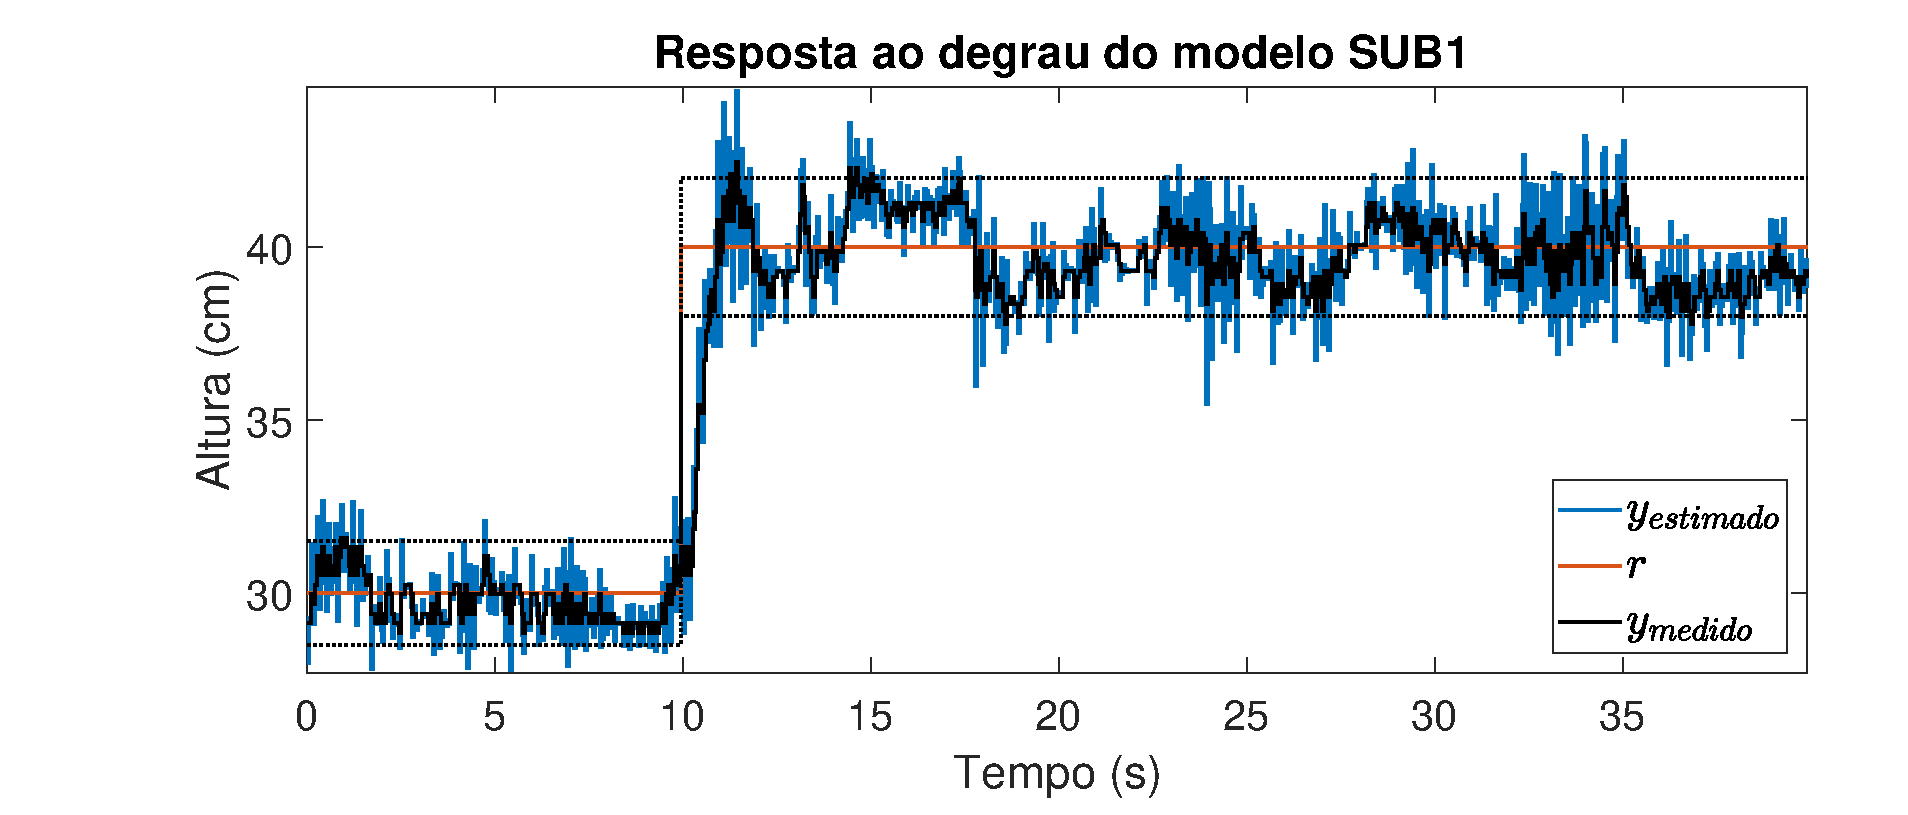
\includegraphics[width=1\linewidth]{steprsub1y}
		\caption[$y_{estimado}$ e $y_{medido}$ do modelo $SUB1$]{$y_{estimado}$ e $y_{medido}$ do modelo $SUB1$}
		\label{fig:steprsub1y}
	\end{subfigure}
	~ %add desired spacing between images, e. g. ~, \quad, \qquad, \hfill etc. 
	%(or a blank line to force the subfigure onto a new line)
	\begin{subfigure}[b]{1\textwidth}
		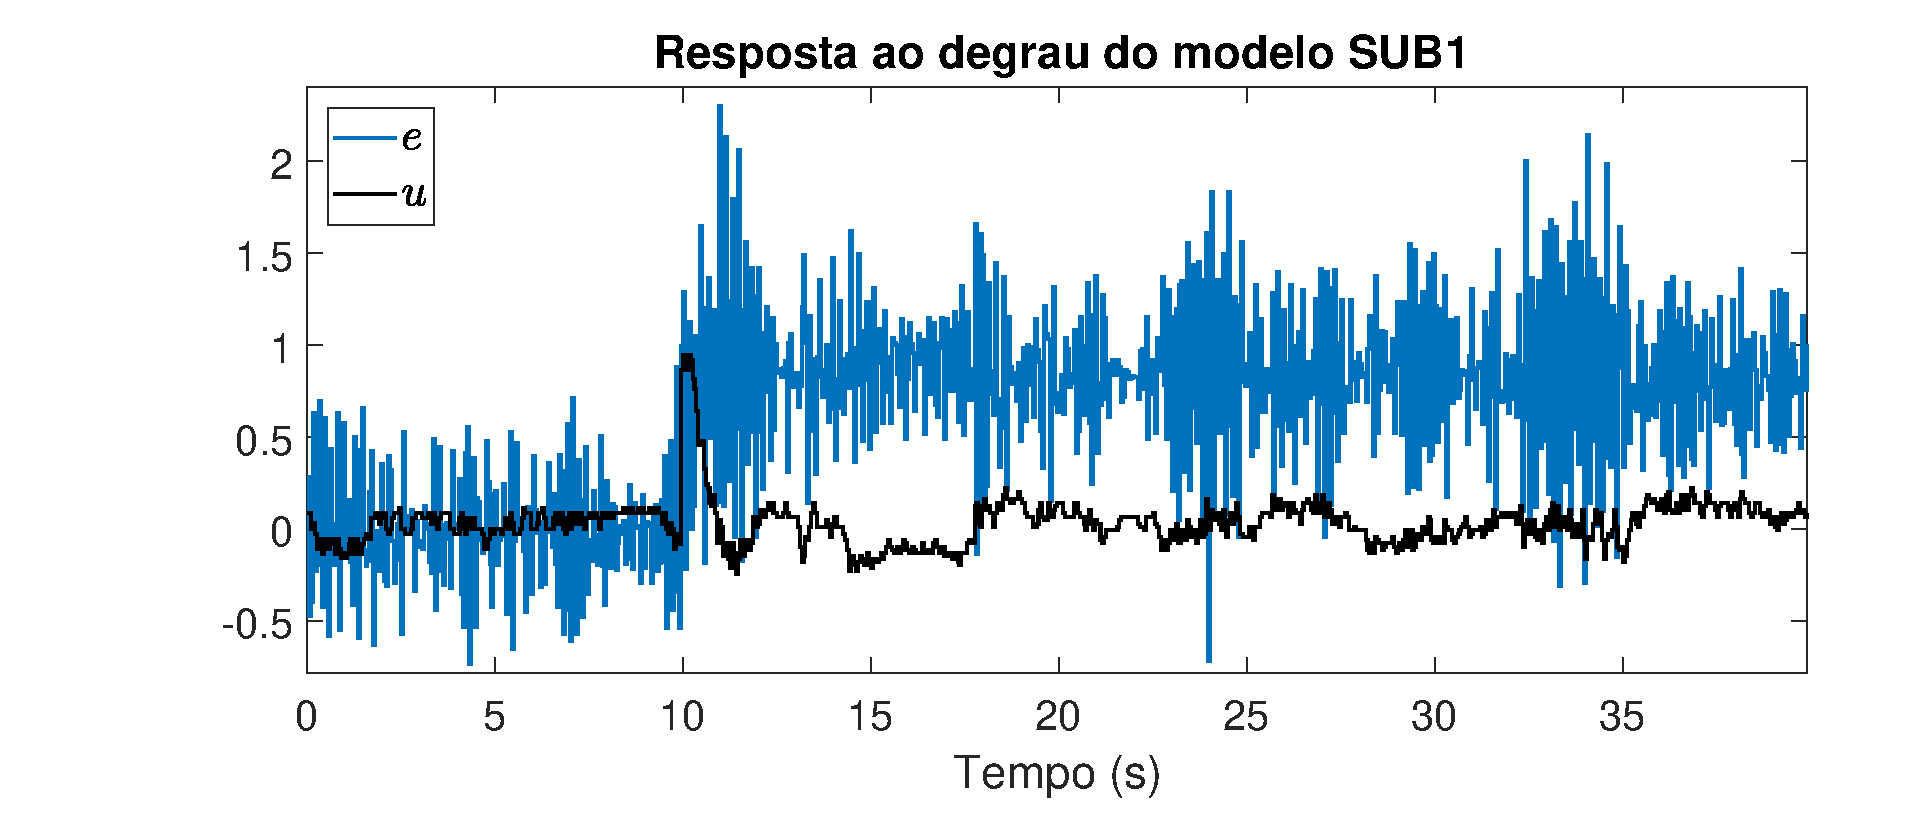
\includegraphics[width=1\linewidth]{steprsub1e}
		\caption[erro $e$ e sinal de controle $u$ do controlador $SUB1$]{erro $e$ e sinal de controle $u$ do controlador $SUB1$}
		\label{fig:steprsub1e}
	\end{subfigure}
	~ %add desired spacing between images, e. g. ~, \quad, \qquad, \hfill etc. 
	%(or a blank line to force the subfigure onto a new line)
	
	\caption{Resposta ao degrau do sistema usando o controlador $SUB1$}\label{fig:steprsub1}
\end{figure}

\begin{figure}[H]
	\centering
	\begin{subfigure}[b]{1\textwidth}
		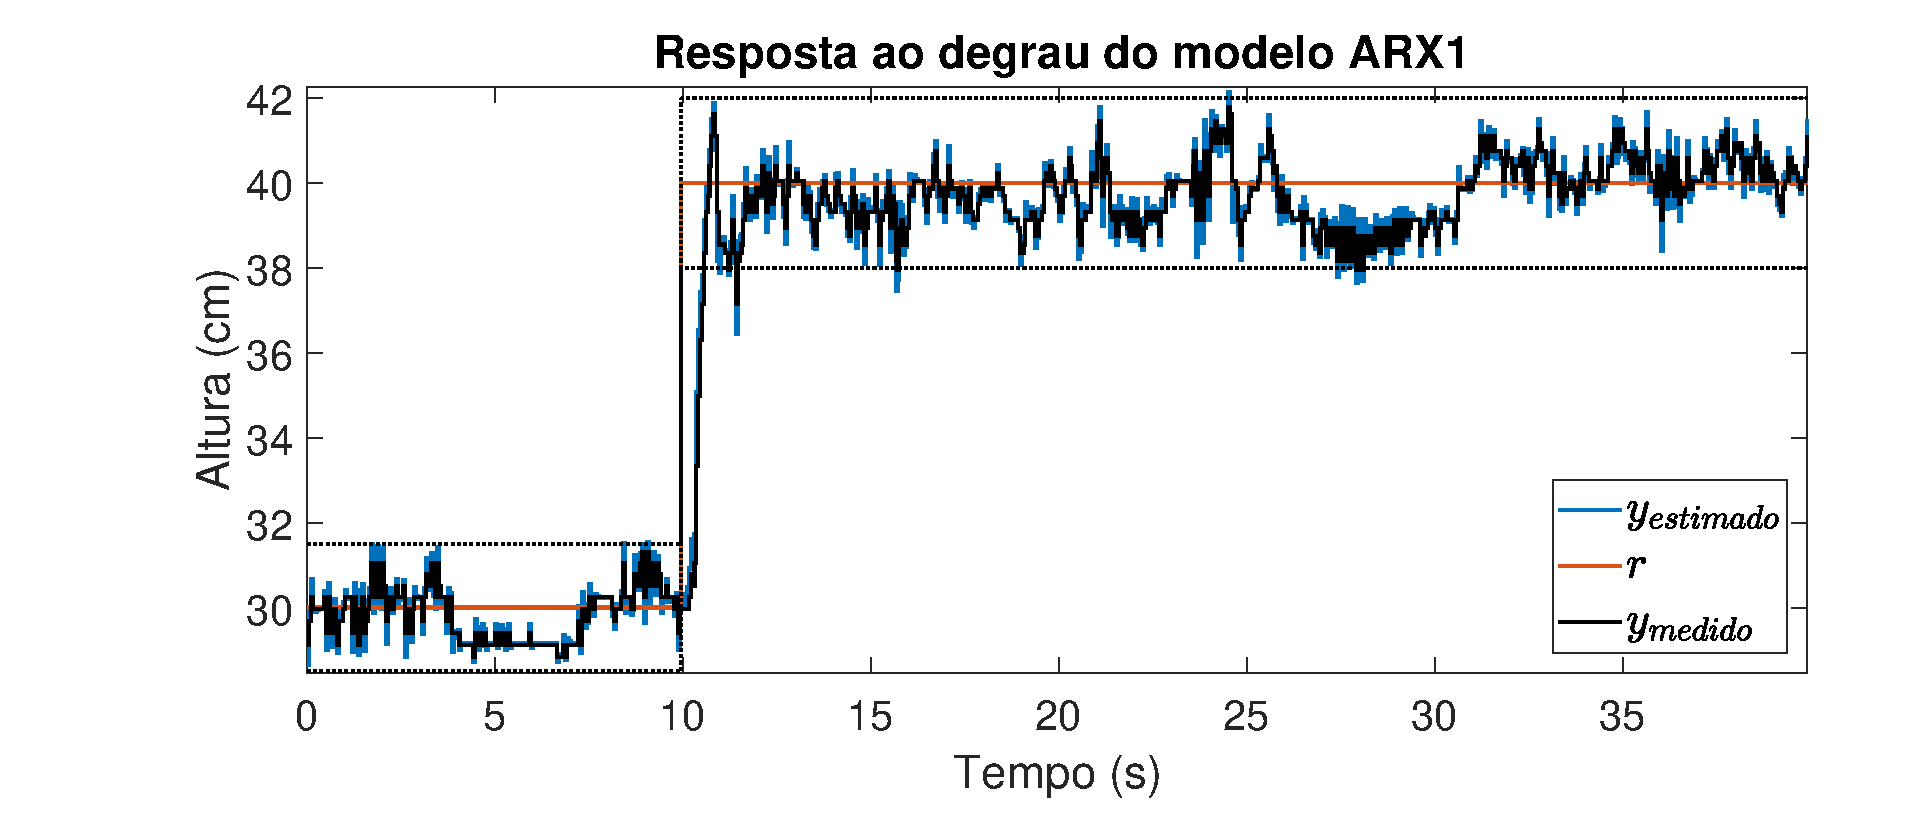
\includegraphics[width=1\linewidth]{steprarx1y}
		\caption[$y_{estimado}$ e $y_{medido}$ do modelo $ARX1$]{$y_{estimado}$ e $y_{medido}$ do modelo $ARX1$}
		\label{fig:steprarx1y}
	\end{subfigure}
	~ %add desired spacing between images, e. g. ~, \quad, \qquad, \hfill etc. 
	%(or a blank line to force the subfigure onto a new line)
	\begin{subfigure}[b]{1\textwidth}
		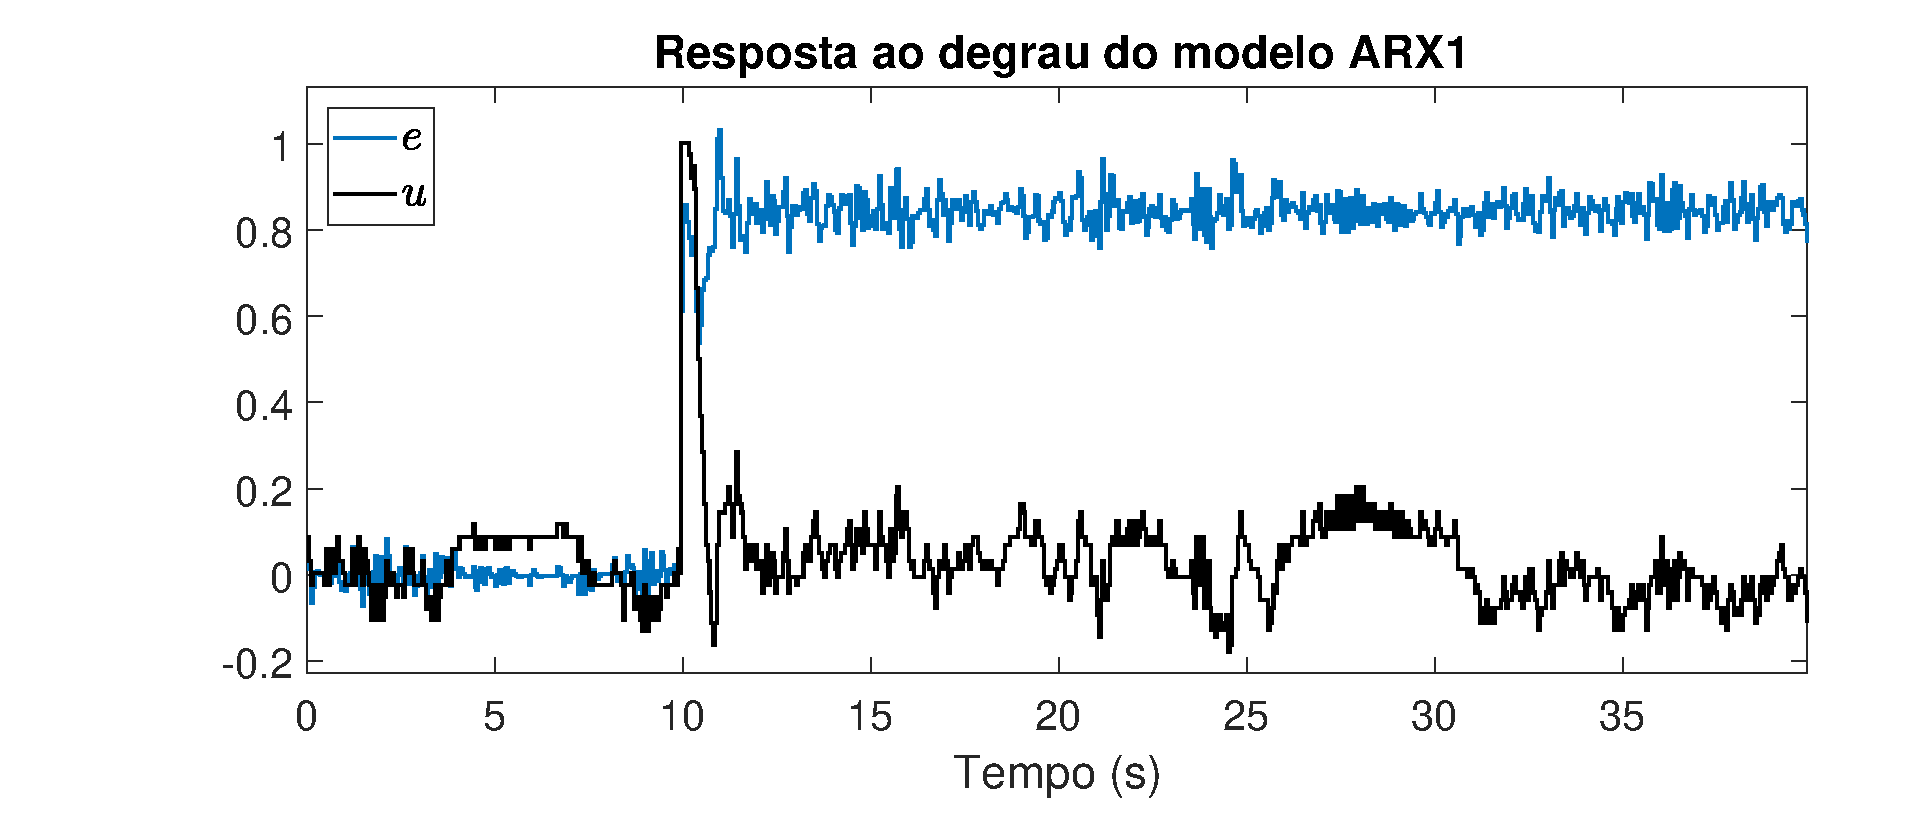
\includegraphics[width=1\linewidth]{steprarx1e}
		\caption[erro $e$ e sinal de controle $u$ do controlador $ARX1$]{erro $e$ e sinal de controle $u$ do controlador $ARX1$}
		\label{fig:steprarx1e}
	\end{subfigure}
	~ %add desired spacing between images, e. g. ~, \quad, \qquad, \hfill etc. 
	%(or a blank line to force the subfigure onto a new line)
	
	\caption{Resposta à perturbação externa do sistema com o controlador do modelo $ARX1$}\label{fig:steprarx1}
\end{figure}

\begin{figure}[H]
	\centering
	\begin{subfigure}[b]{1\textwidth}
		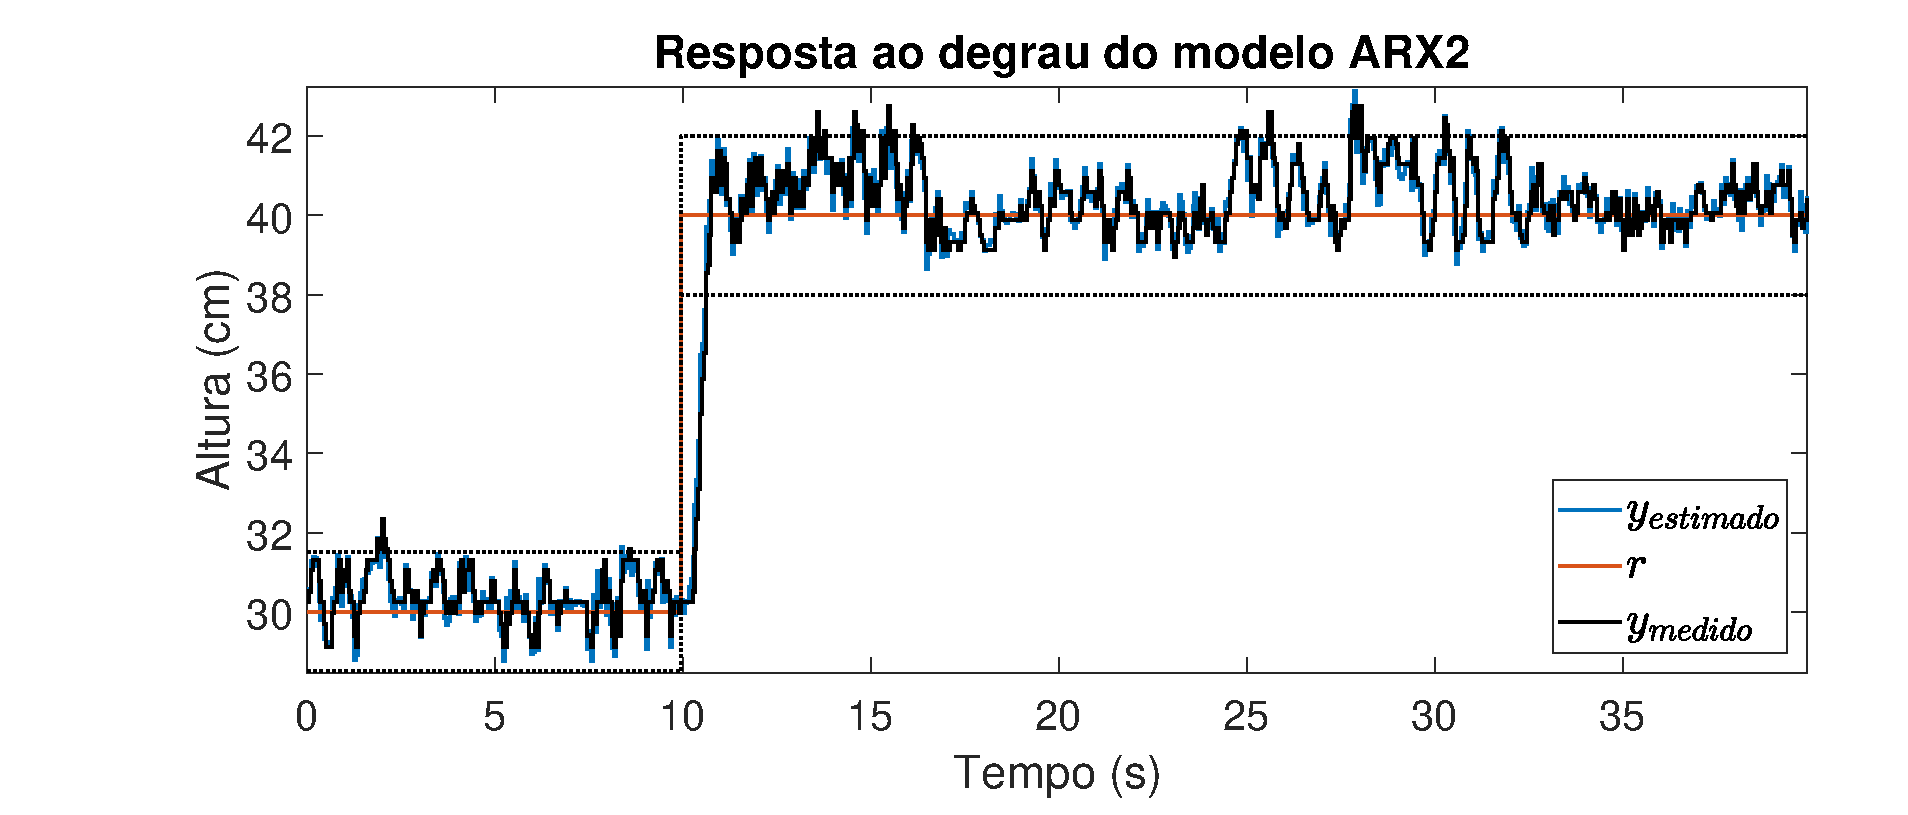
\includegraphics[width=1\linewidth]{steprarx2y}
		\caption[$y_{estimado}$ e $y_{medido}$ do modelo $ARX2$]{$y_{estimado}$ e $y_{medido}$ do modelo $ARX2$}
		\label{fig:steprarx2y}
	\end{subfigure}
	~ %add desired spacing between images, e. g. ~, \quad, \qquad, \hfill etc. 
	%(or a blank line to force the subfigure onto a new line)
	\begin{subfigure}[b]{1\textwidth}
		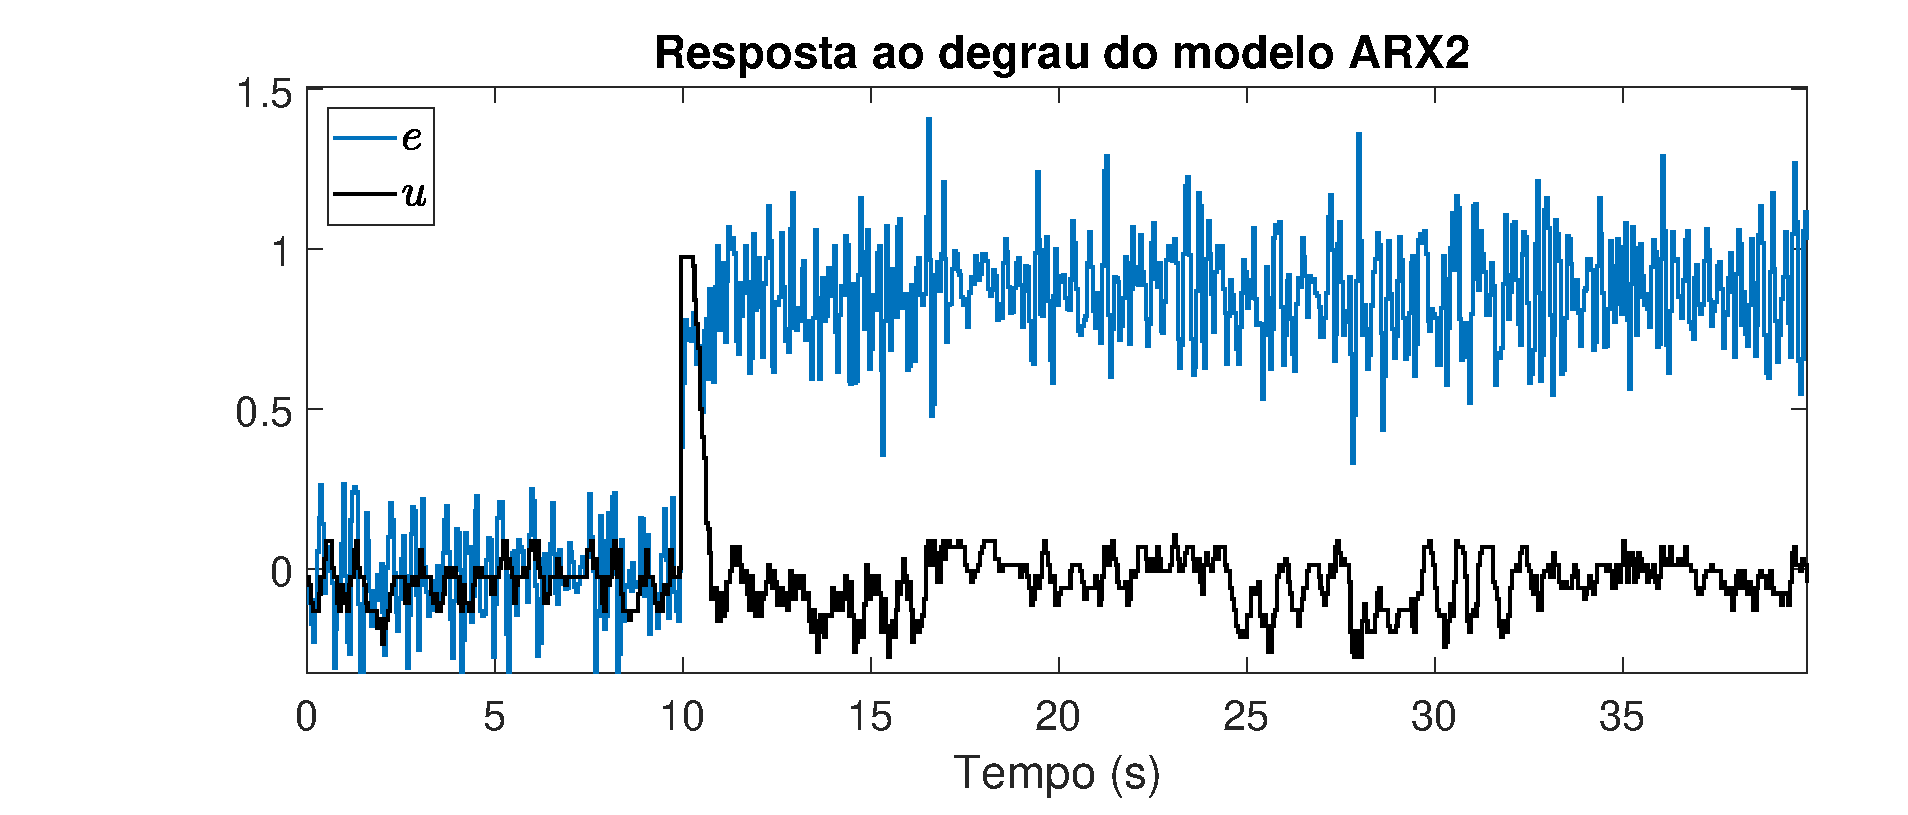
\includegraphics[width=1\linewidth]{steprarx2e}
		\caption[erro $e$ e sinal de controle $u$ do controlador $ARX2$]{erro $e$ e sinal de controle $u$ do controlador $ARX2$}
		\label{fig:steprarx2e}
	\end{subfigure}
	~ %add desired spacing between images, e. g. ~, \quad, \qquad, \hfill etc. 
	%(or a blank line to force the subfigure onto a new line)
	
	\caption{Resposta à perturbação externa do sistema com o controlador do modelo $ARX2$}\label{fig:steprarx2}
\end{figure}

\subsection{Resultados da Resposta à escadaria}\label{rstair}
\begin{figure}[H]
	\centering
	\begin{subfigure}[b]{1\textwidth}
		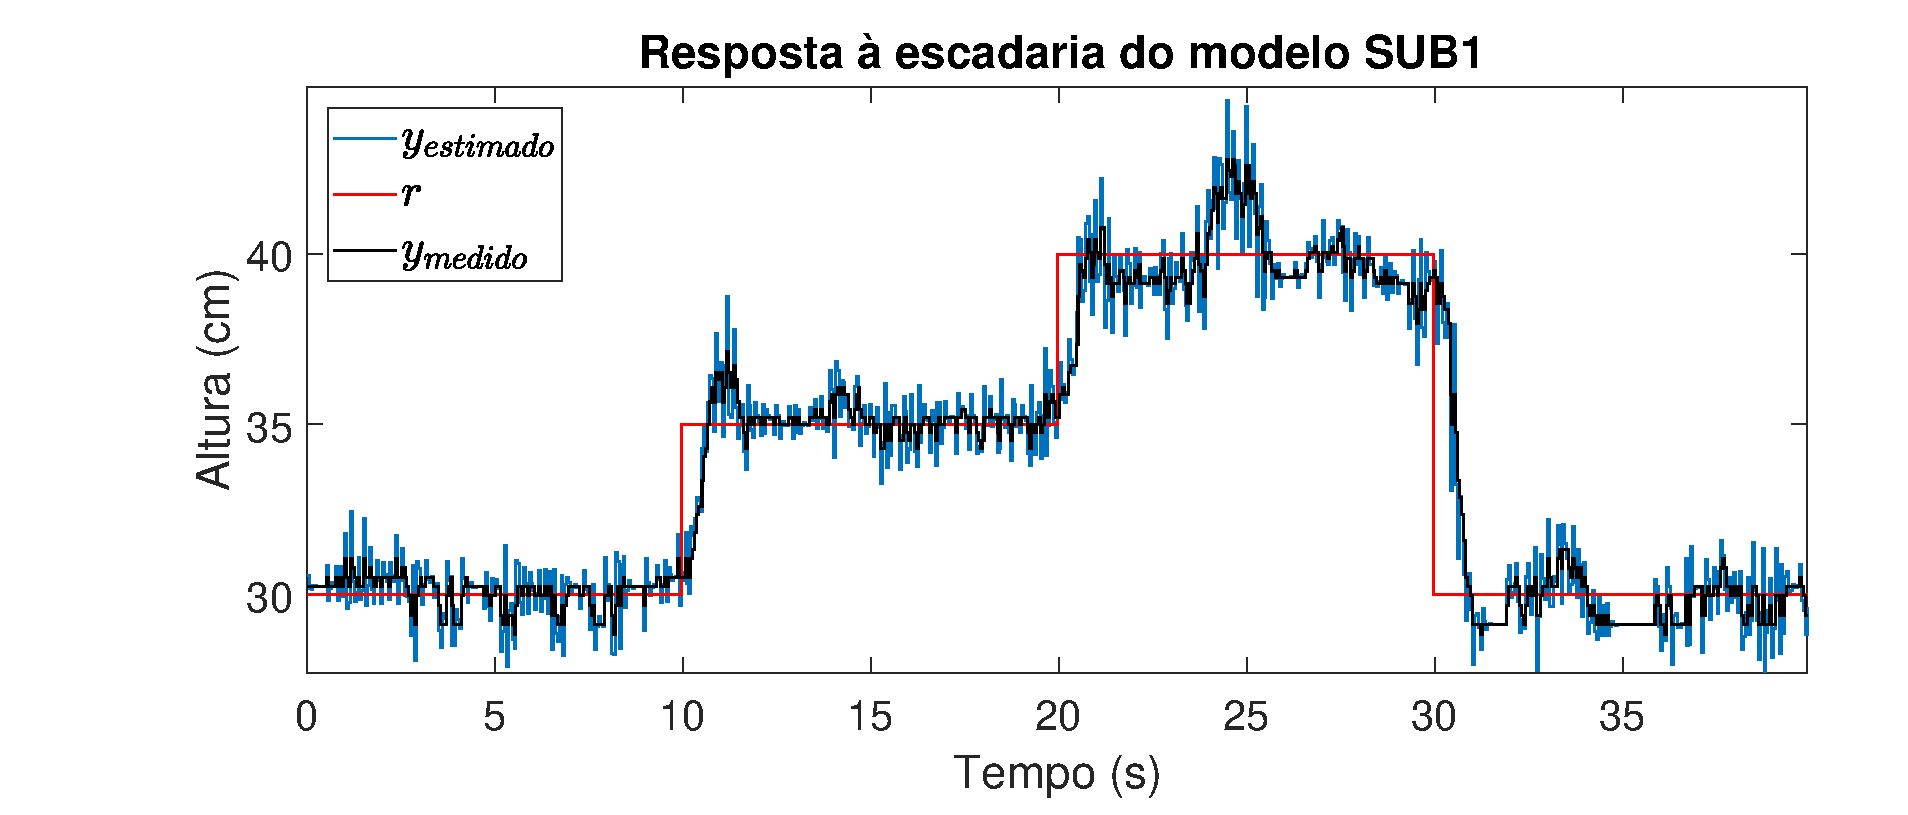
\includegraphics[width=1\linewidth]{stairrsub1y}
		\caption[$y_{estimado}$ e $y_{medido}$ do modelo $SUB1$]{$y_{estimado}$ e $y_{medido}$ do modelo $SUB1$}
		\label{fig:stairrsub1y}
	\end{subfigure}
	~ %add desired spacing between images, e. g. ~, \quad, \qquad, \hfill etc. 
	%(or a blank line to force the subfigure onto a new line)
	\begin{subfigure}[b]{1\textwidth}
		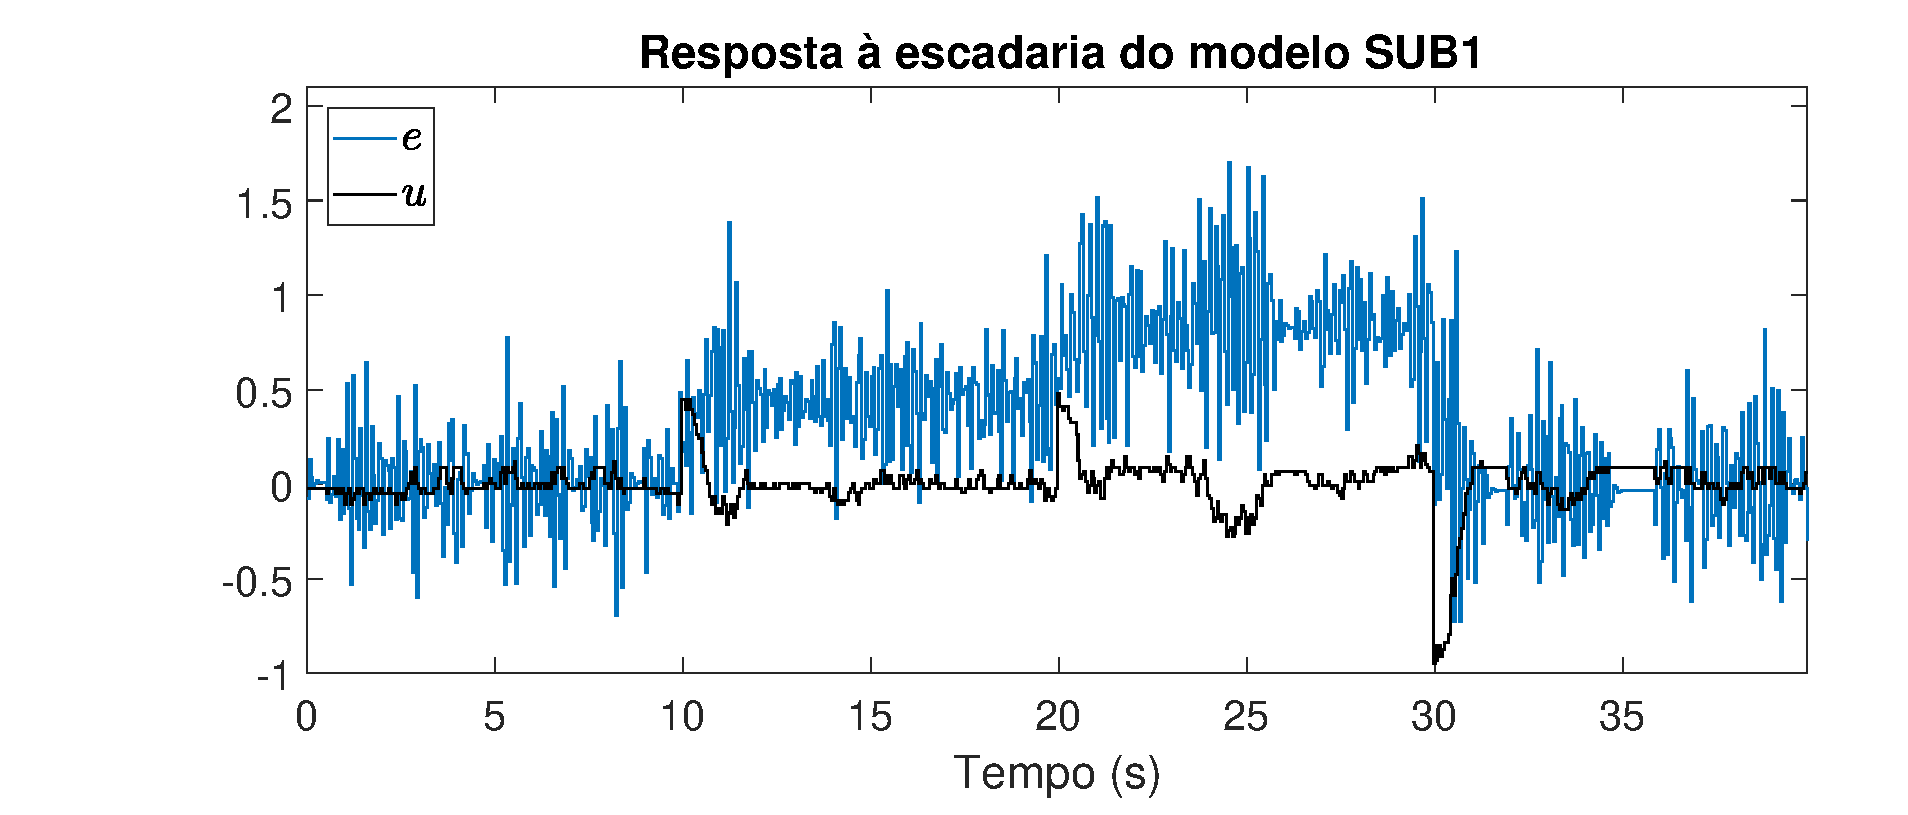
\includegraphics[width=1\linewidth]{stairrsub1e}
		\caption[erro $e$ e sinal de controle $u$ do controlador $SUB1$]{erro $e$ e sinal de controle $u$ do controlador $SUB1$}
		\label{fig:stairrsub1e}
	\end{subfigure}
	~ %add desired spacing between images, e. g. ~, \quad, \qquad, \hfill etc. 
	%(or a blank line to force the subfigure onto a new line)
	
	\caption{Resposta à perturbação externa do sistema com o controlador do modelo $SUB1$}\label{fig:stairrsub1}
\end{figure}

\begin{figure}[H]
	\centering
	\begin{subfigure}[b]{1\textwidth}
		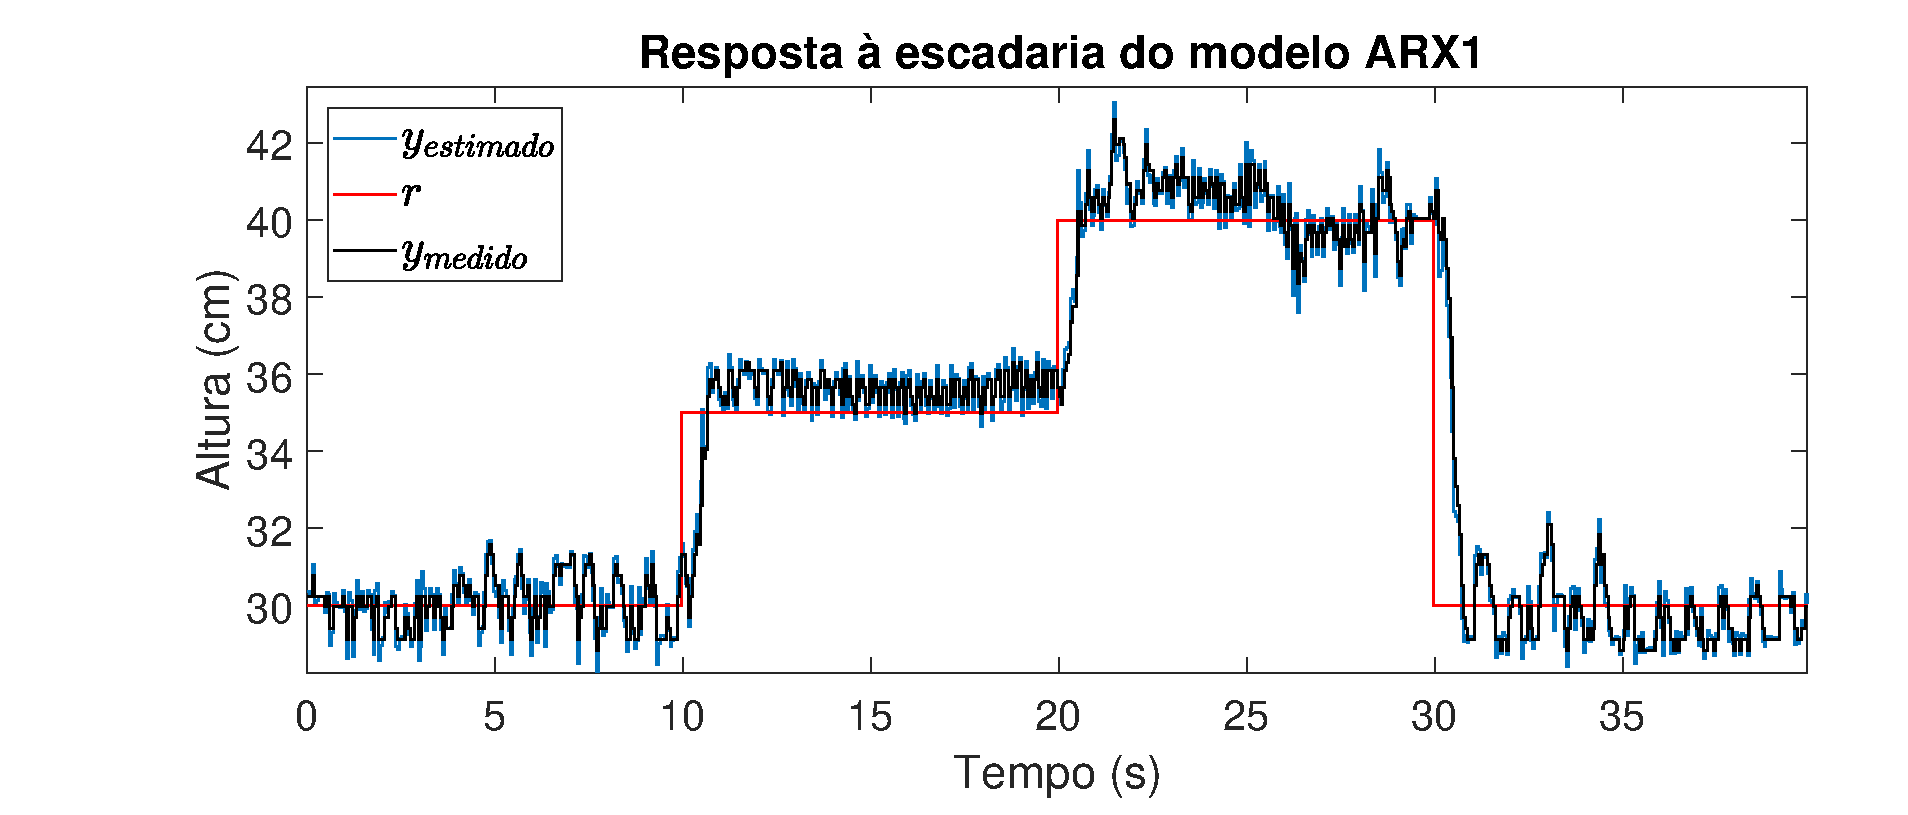
\includegraphics[width=1\linewidth]{stairrarx1y}
		\caption[$y_{estimado}$ e $y_{medido}$ do modelo $ARX1$]{$y_{estimado}$ e $y_{medido}$ do modelo $ARX1$}
		\label{fig:stairrarx1y}
	\end{subfigure}
	~ %add desired spacing between images, e. g. ~, \quad, \qquad, \hfill etc. 
	%(or a blank line to force the subfigure onto a new line)
	\begin{subfigure}[b]{1\textwidth}
		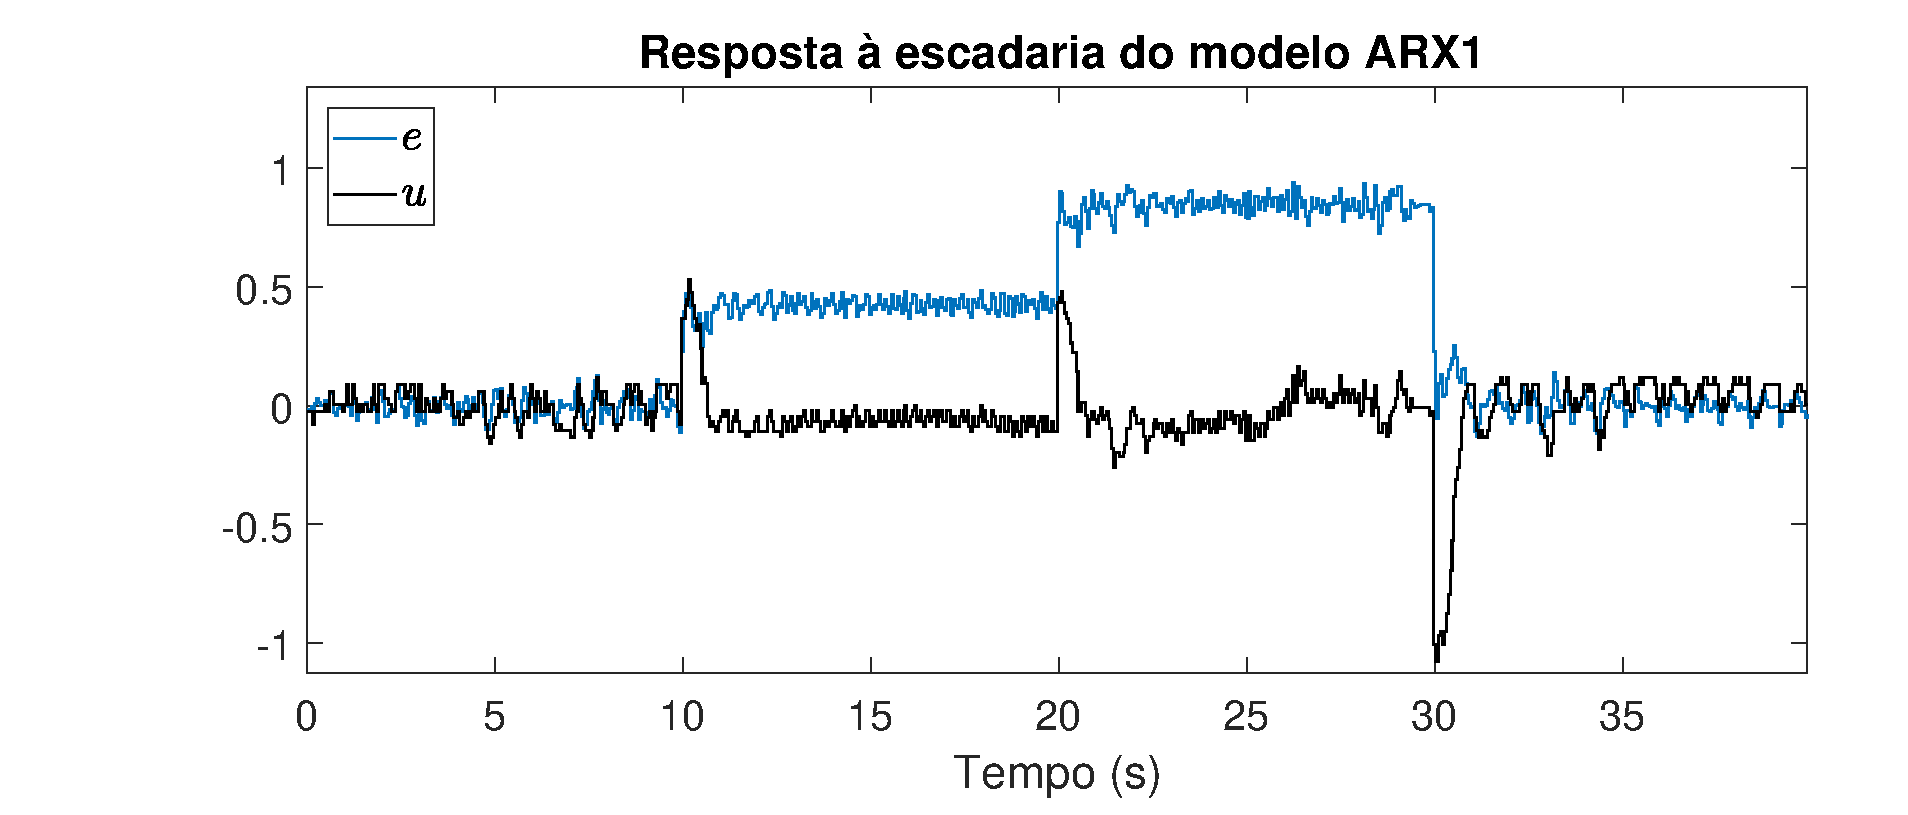
\includegraphics[width=1\linewidth]{stairrarx1e}
		\caption[erro $e$ e sinal de controle $u$ do controlador $ARX1$]{erro $e$ e sinal de controle $u$ do controlador $ARX1$}
		\label{fig:stairrarx1e}
	\end{subfigure}
	~ %add desired spacing between images, e. g. ~, \quad, \qquad, \hfill etc. 
	%(or a blank line to force the subfigure onto a new line)
	
	\caption{Resposta à perturbação externa do sistema com o controlador do modelo $ARX1$}\label{fig:stairrarx1}
\end{figure}

\begin{figure}[H]
	\centering
	\begin{subfigure}[b]{1\textwidth}
		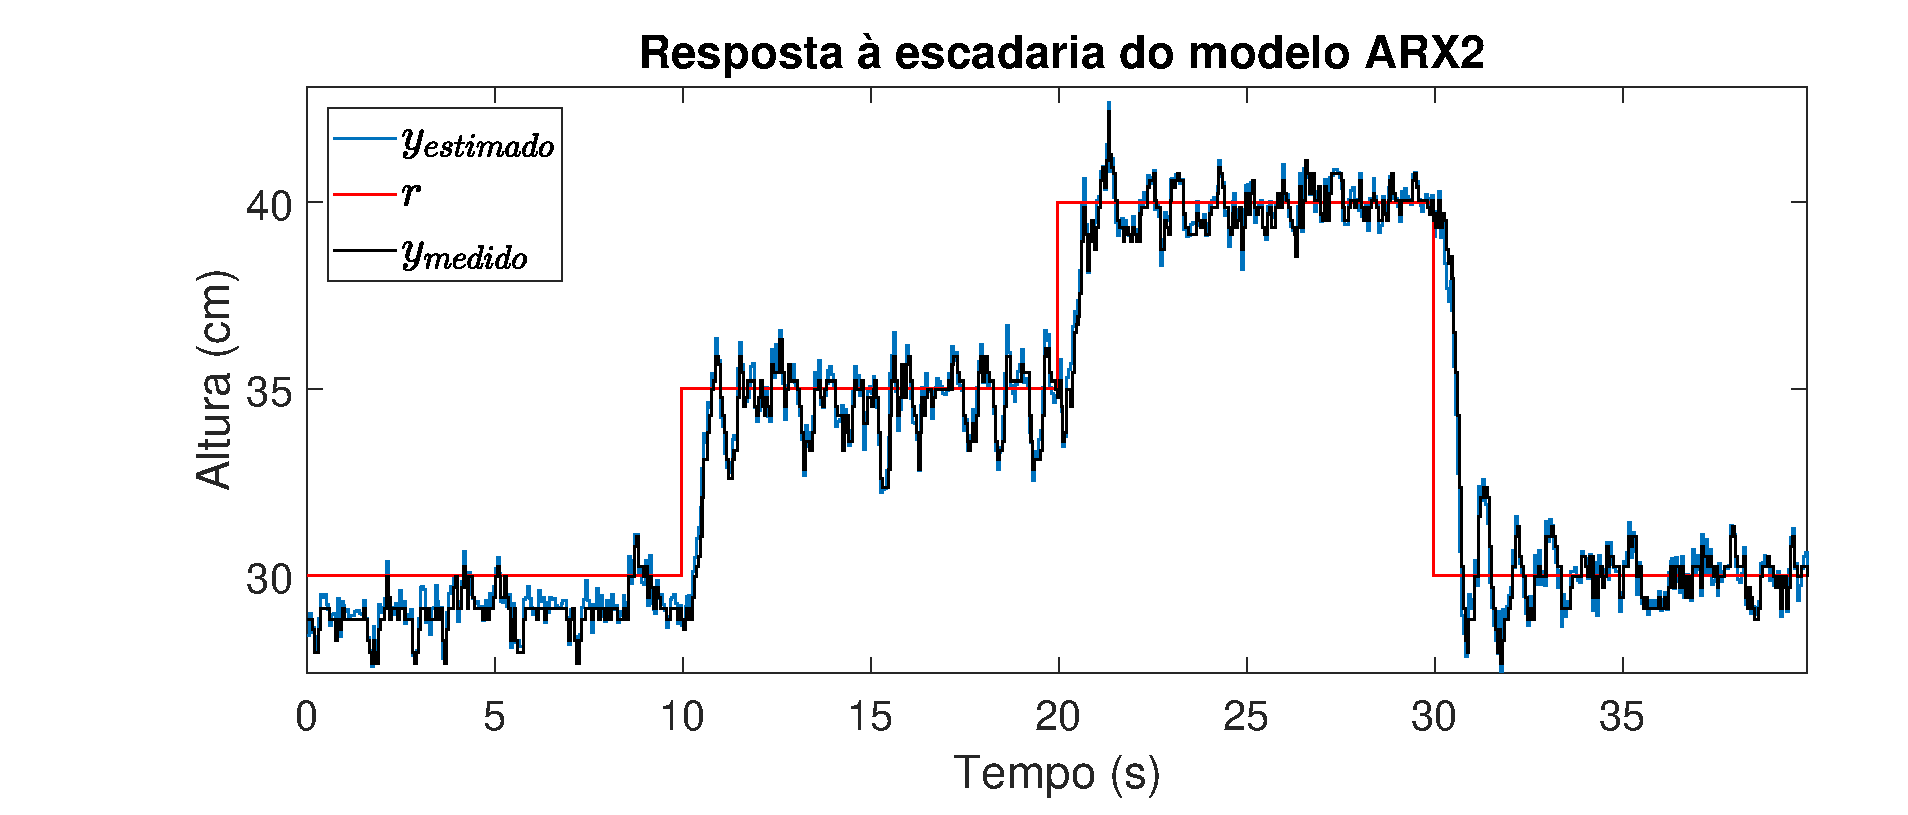
\includegraphics[width=1\linewidth]{stairrarx2y}
		\caption[$y_{estimado}$ e $y_{medido}$ do modelo $ARX2$]{$y_{estimado}$ e $y_{medido}$ do modelo $ARX2$}
		\label{fig:stairrarx2y}
	\end{subfigure}
	~ %add desired spacing between images, e. g. ~, \quad, \qquad, \hfill etc. 
	%(or a blank line to force the subfigure onto a new line)
	\begin{subfigure}[b]{1\textwidth}
		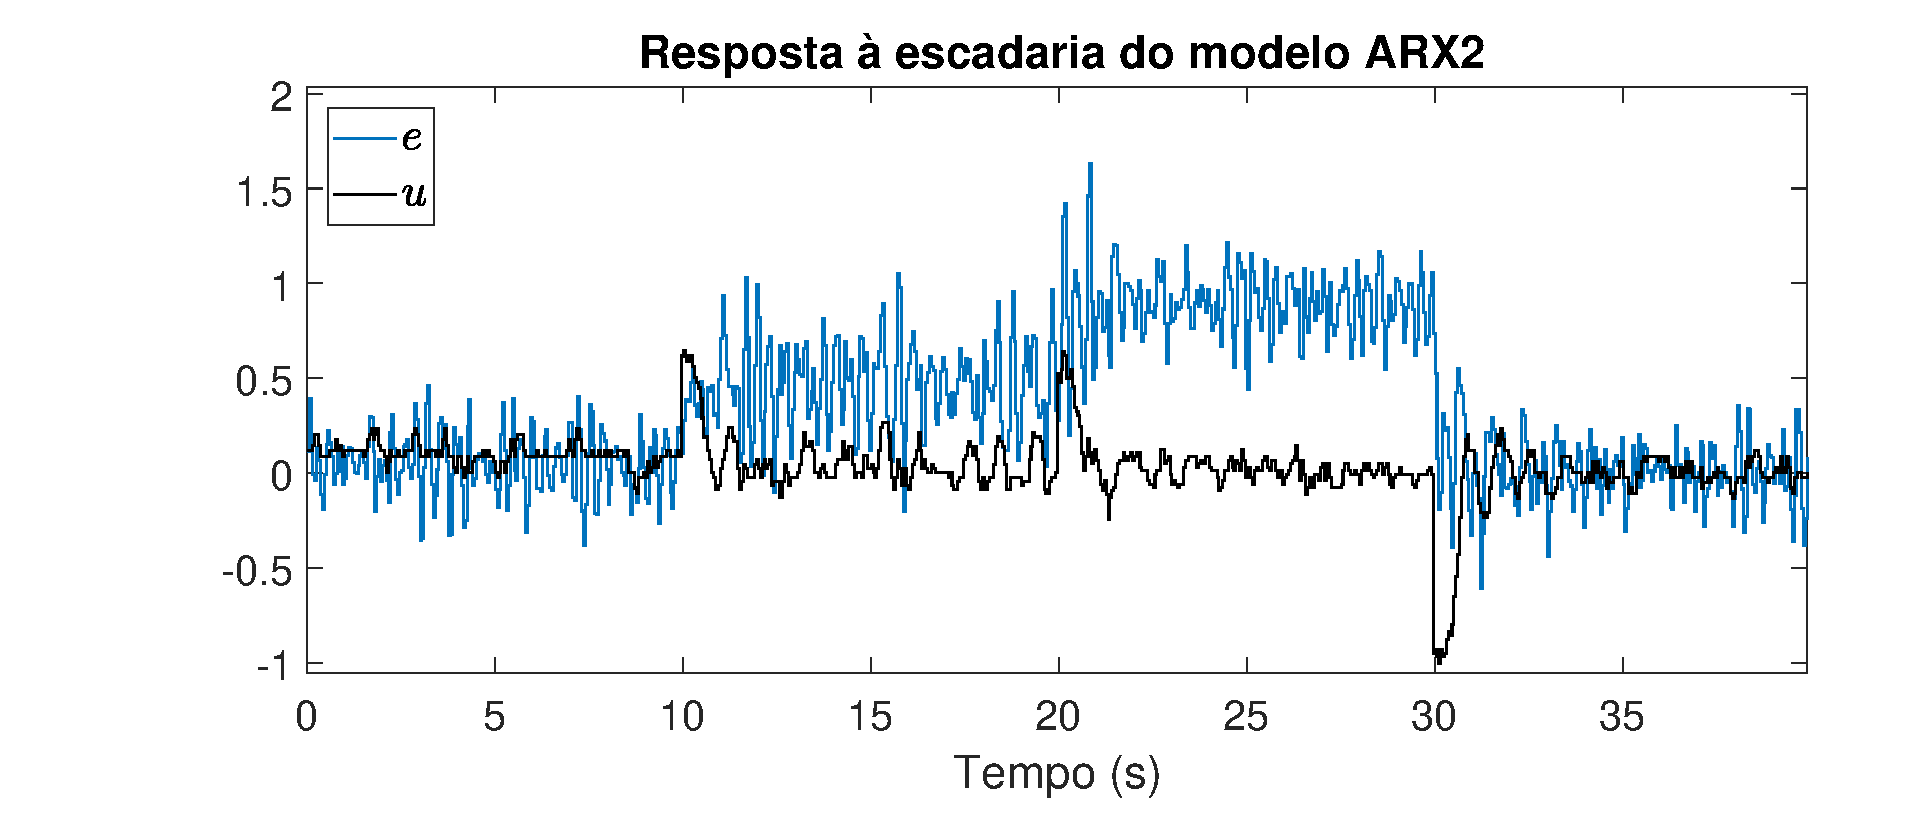
\includegraphics[width=1\linewidth]{stairrarx2e}
		\caption[erro $e$ e sinal de controle $u$ do controlador $ARX2$]{erro $e$ e sinal de controle $u$ do controlador $ARX2$}
		\label{fig:stairrarx2e}
	\end{subfigure}
	~ %add desired spacing between images, e. g. ~, \quad, \qquad, \hfill etc. 
	%(or a blank line to force the subfigure onto a new line)
	
	\caption{Resposta à perturbação externa do sistema com o controlador do modelo $ARX2$}\label{fig:stairrarx2}
\end{figure}

\subsubsection{Erro do Estimador} \label{erroest}

\begin{figure}
	\centering
	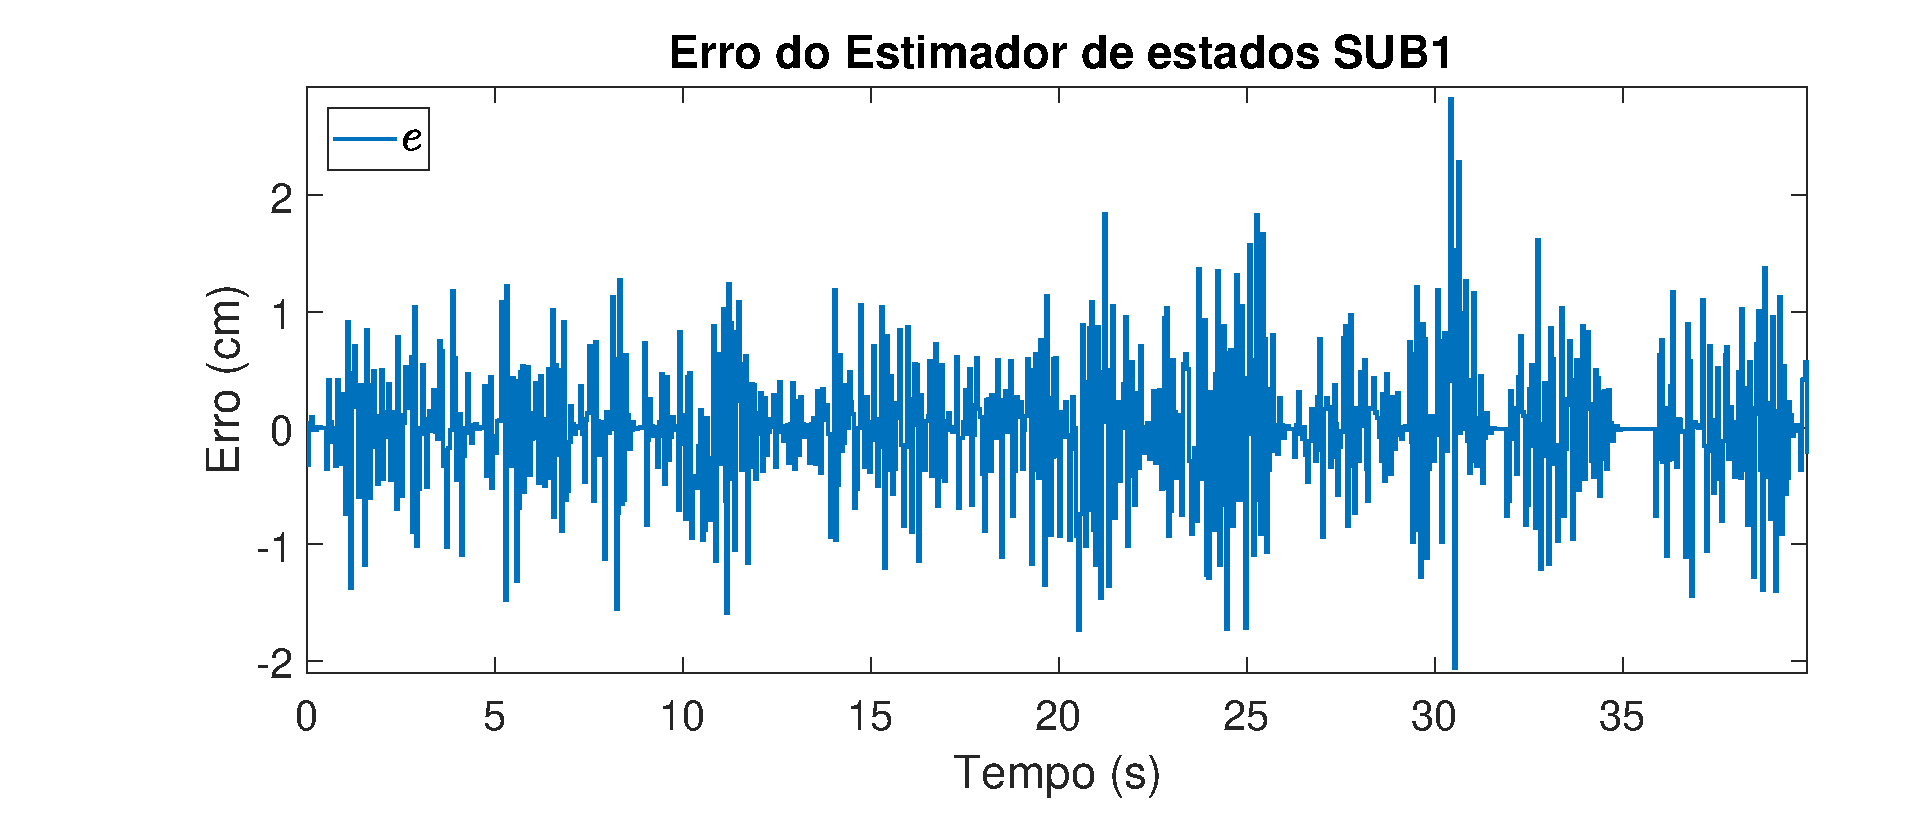
\includegraphics[width=1\linewidth]{errosub1}
	\caption[Erro do estimador do modelo $SUB1$ na resposta à escadaria]{Erro do estimador do modelo $SUB1$ na resposta à escadaria}
	\label{fig:errosub1}
\end{figure}

\begin{figure}
	\centering
	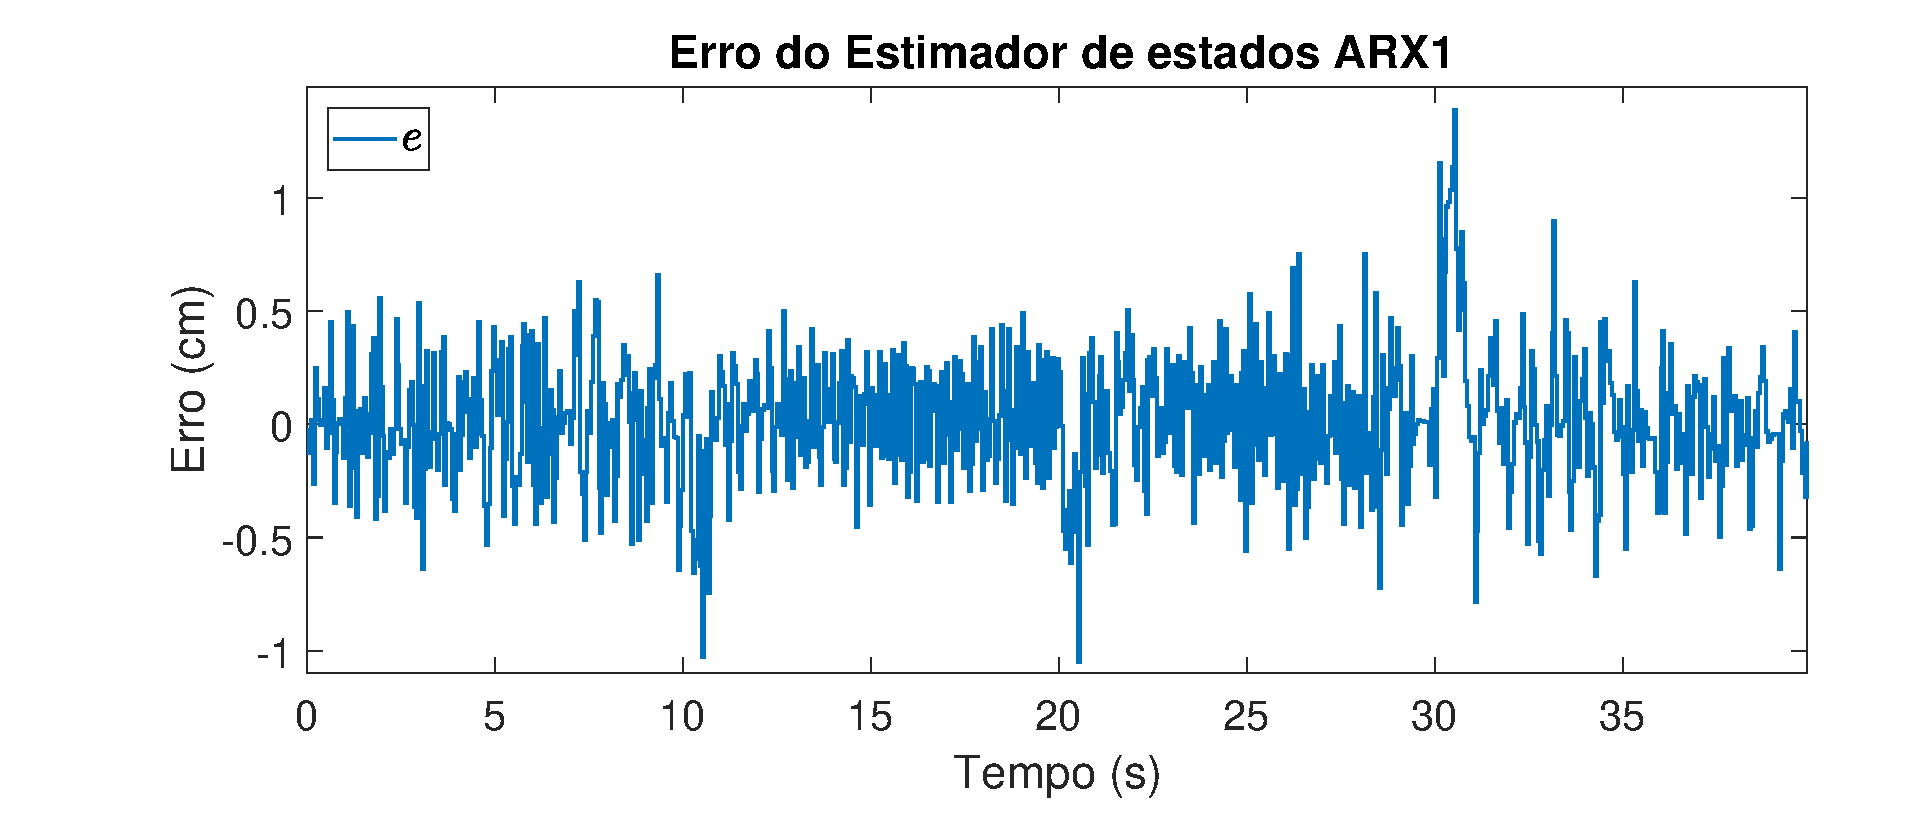
\includegraphics[width=1\linewidth]{erroarx1}
	\caption[Erro do estimador do modelo $ARX1$ na resposta à escadaria]{Erro do estimador do modelo $ARX1$ na resposta à escadaria}
	\label{fig:erroarx1}
\end{figure}

\begin{figure}
	\centering
	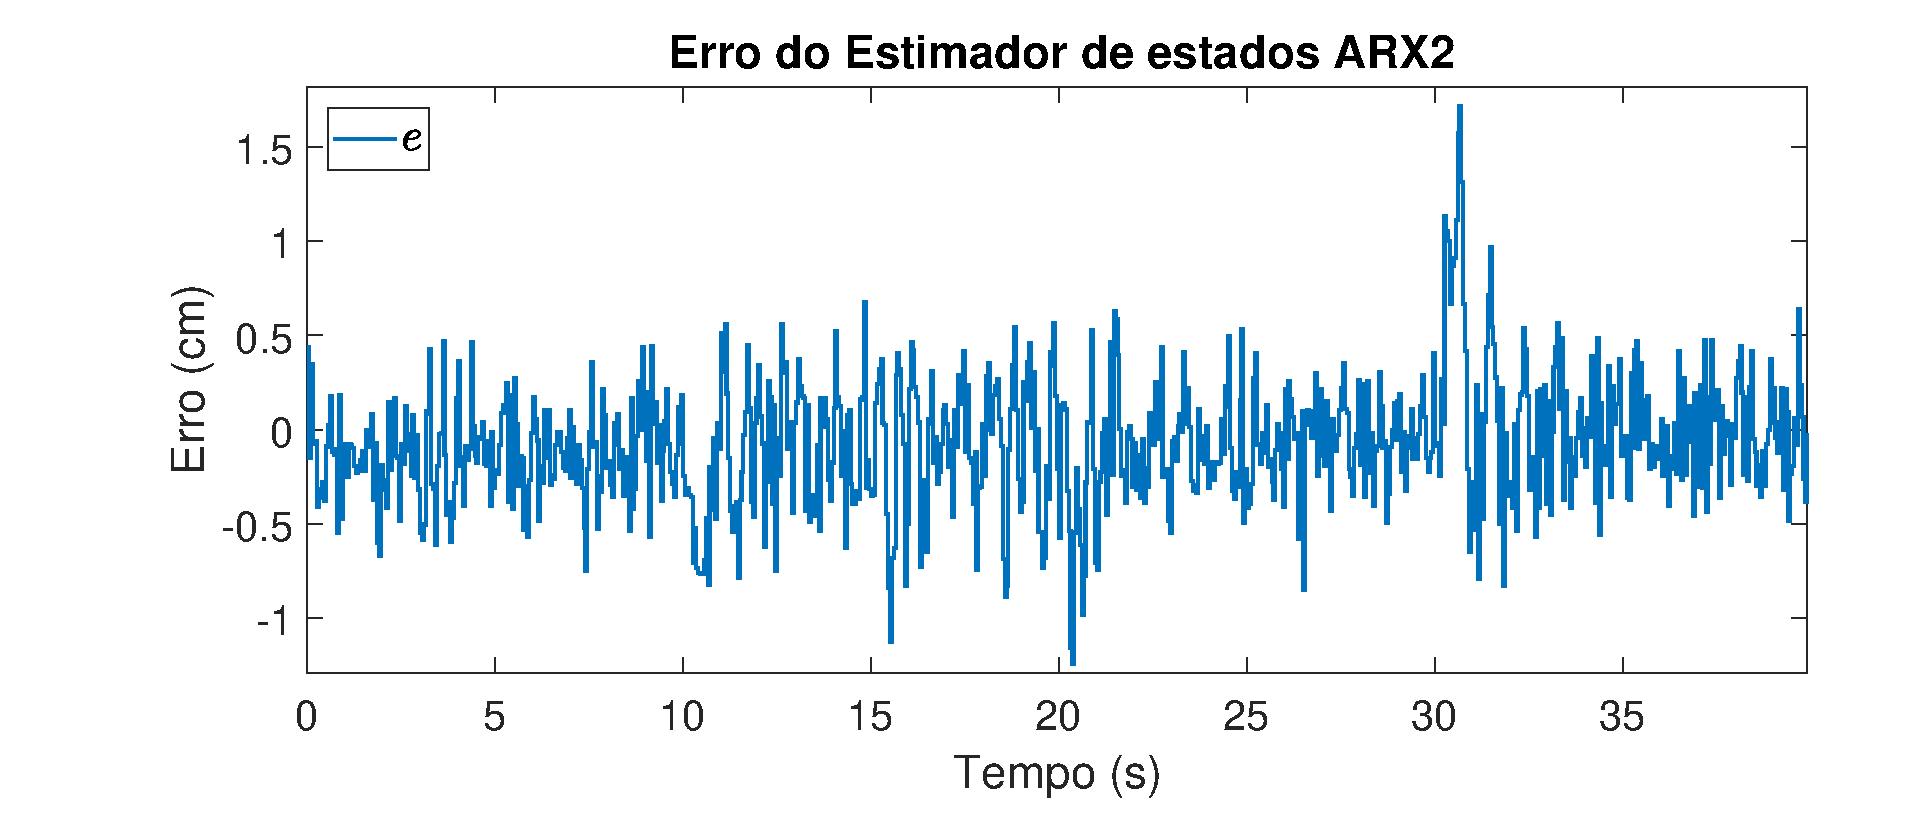
\includegraphics[width=1\linewidth]{erroarx2}
	\caption[Erro do estimador do modelo $ARX2$ na resposta à escadaria]{Erro do estimador do modelo $ARX2$ na resposta à escadaria}
	\label{fig:erroarx2}
\end{figure}


\subsection{Resultados do Teste de Robustez à mudança de Parâmetros}\label{rmp}

\begin{figure}[H]
	\centering
	\begin{subfigure}[b]{1\textwidth}
		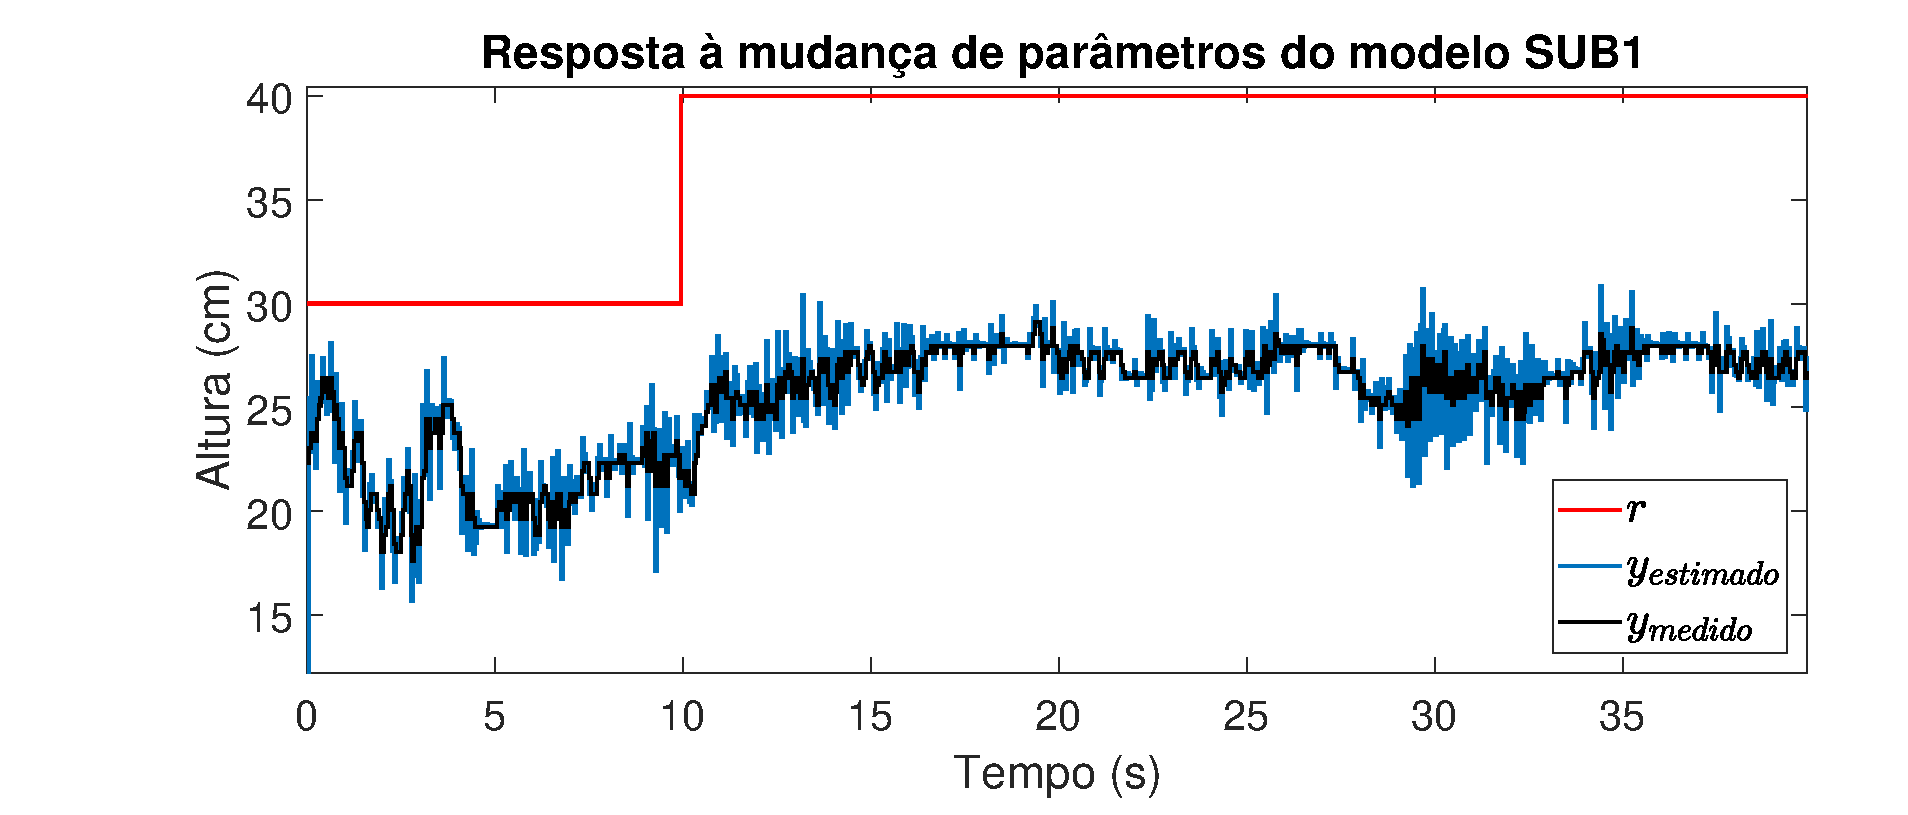
\includegraphics[width=1\linewidth]{mprsub1y}
		\caption[$y_{estimado}$ e $y_{medido}$ do modelo $SUB1$]{$y_{estimado}$ e $y_{medido}$ do modelo $SUB1$}
		\label{fig:mprsub1y}
	\end{subfigure}
	~ %add desired spacing between images, e. g. ~, \quad, \qquad, \hfill etc. 
	%(or a blank line to force the subfigure onto a new line)
	\begin{subfigure}[b]{1\textwidth}
		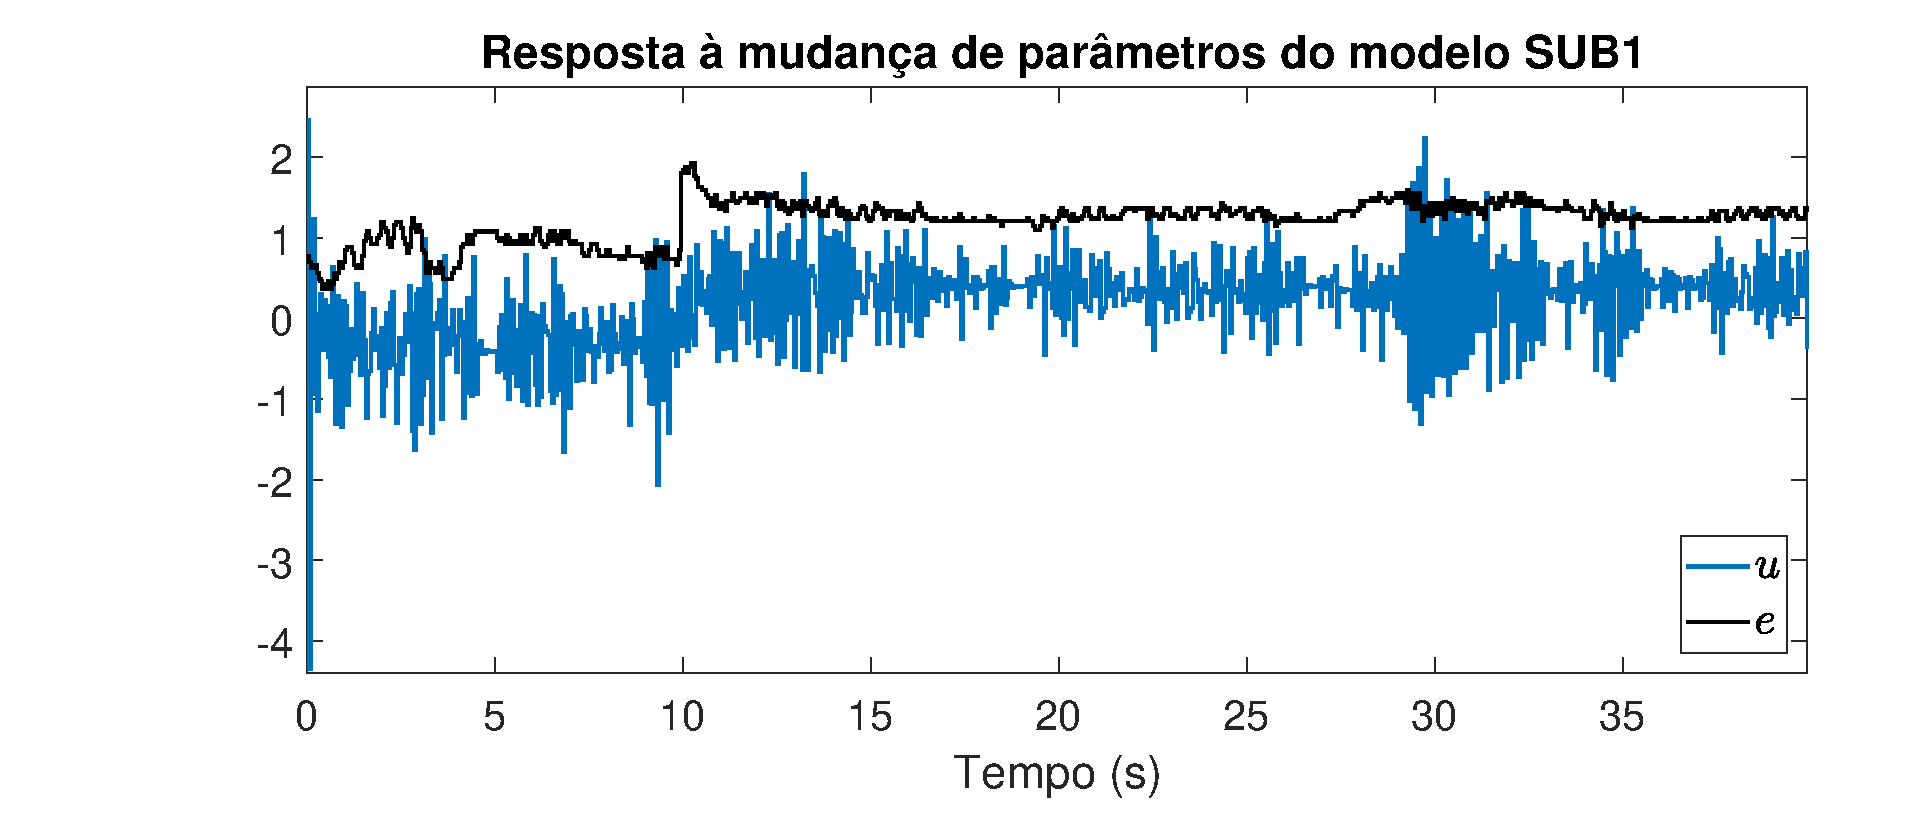
\includegraphics[width=1\linewidth]{mprsub1e}
		\caption[erro $e$ e sinal de controle $u$ do controlador $SUB1$]{erro $e$ e sinal de controle $u$ do controlador $SUB1$}
		\label{fig:mprsub1e}
	\end{subfigure}
	~ %add desired spacing between images, e. g. ~, \quad, \qquad, \hfill etc. 
	%(or a blank line to force the subfigure onto a new line)
	
	\caption{Resposta à perturbação externa do sistema com o controlador do modelo $SUB1$}\label{fig:mprsub1}
\end{figure}

\begin{figure}[H]
	\centering
	\begin{subfigure}[b]{1\textwidth}
		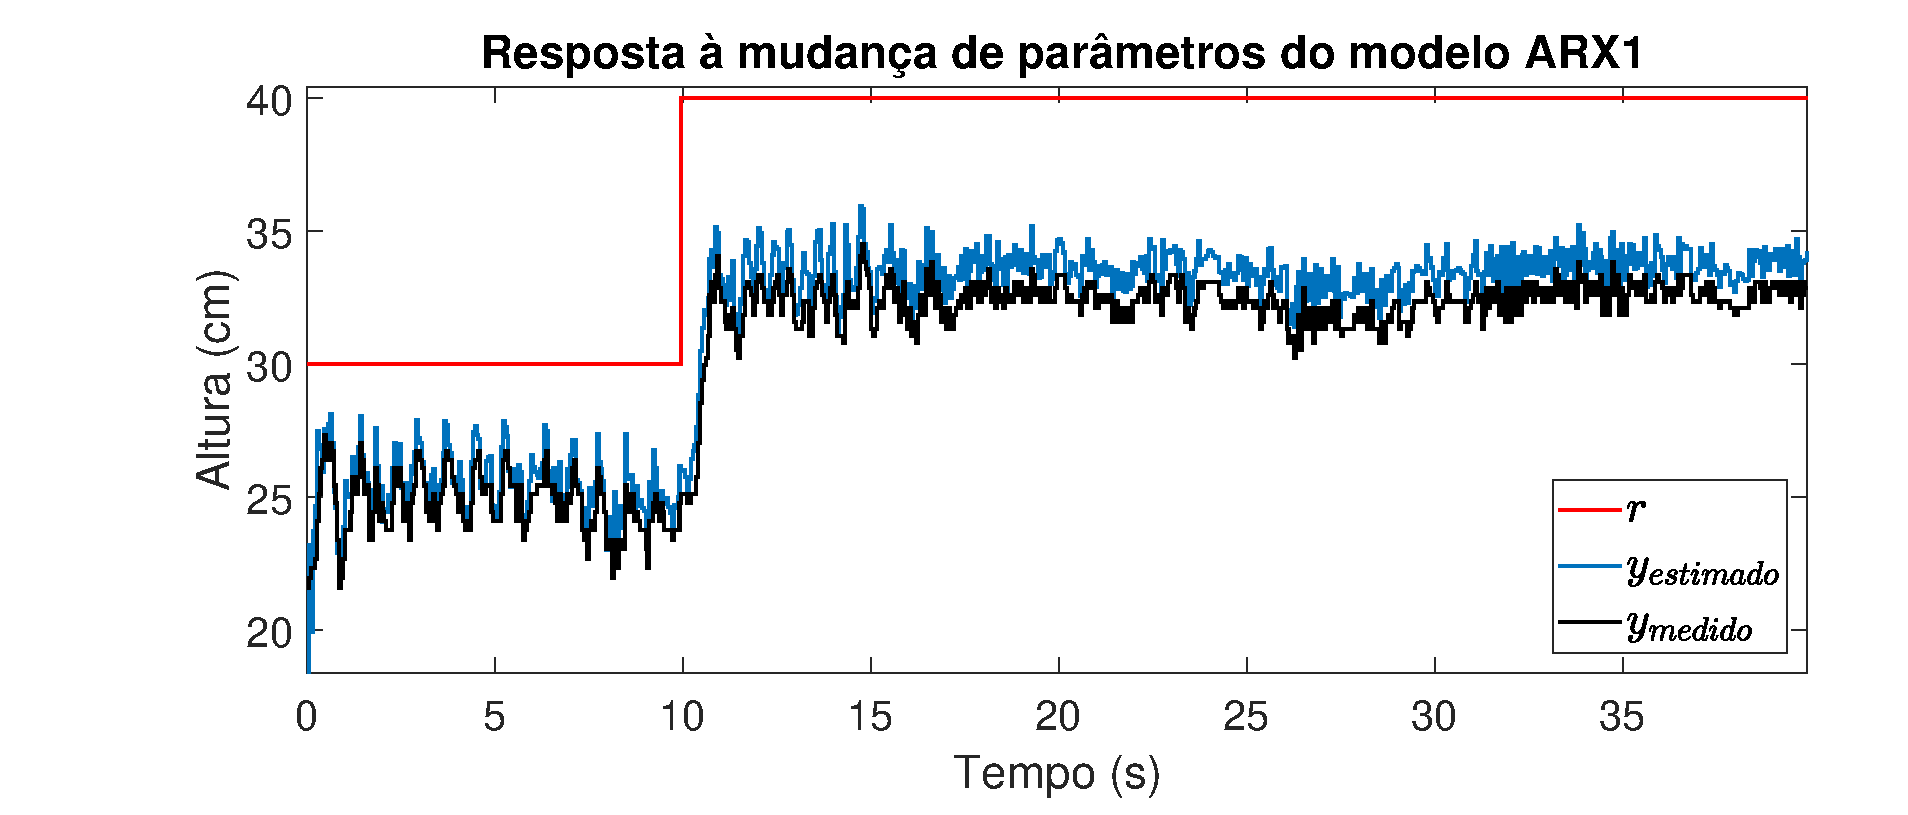
\includegraphics[width=1\linewidth]{mprarx1y}
		\caption[$y_{estimado}$ e $y_{medido}$ do modelo $ARX1$]{$y_{estimado}$ e $y_{medido}$ do modelo $ARX1$}
		\label{fig:mprarx1y}
	\end{subfigure}
	~ %add desired spacing between images, e. g. ~, \quad, \qquad, \hfill etc. 
	%(or a blank line to force the subfigure onto a new line)
	\begin{subfigure}[b]{1\textwidth}
		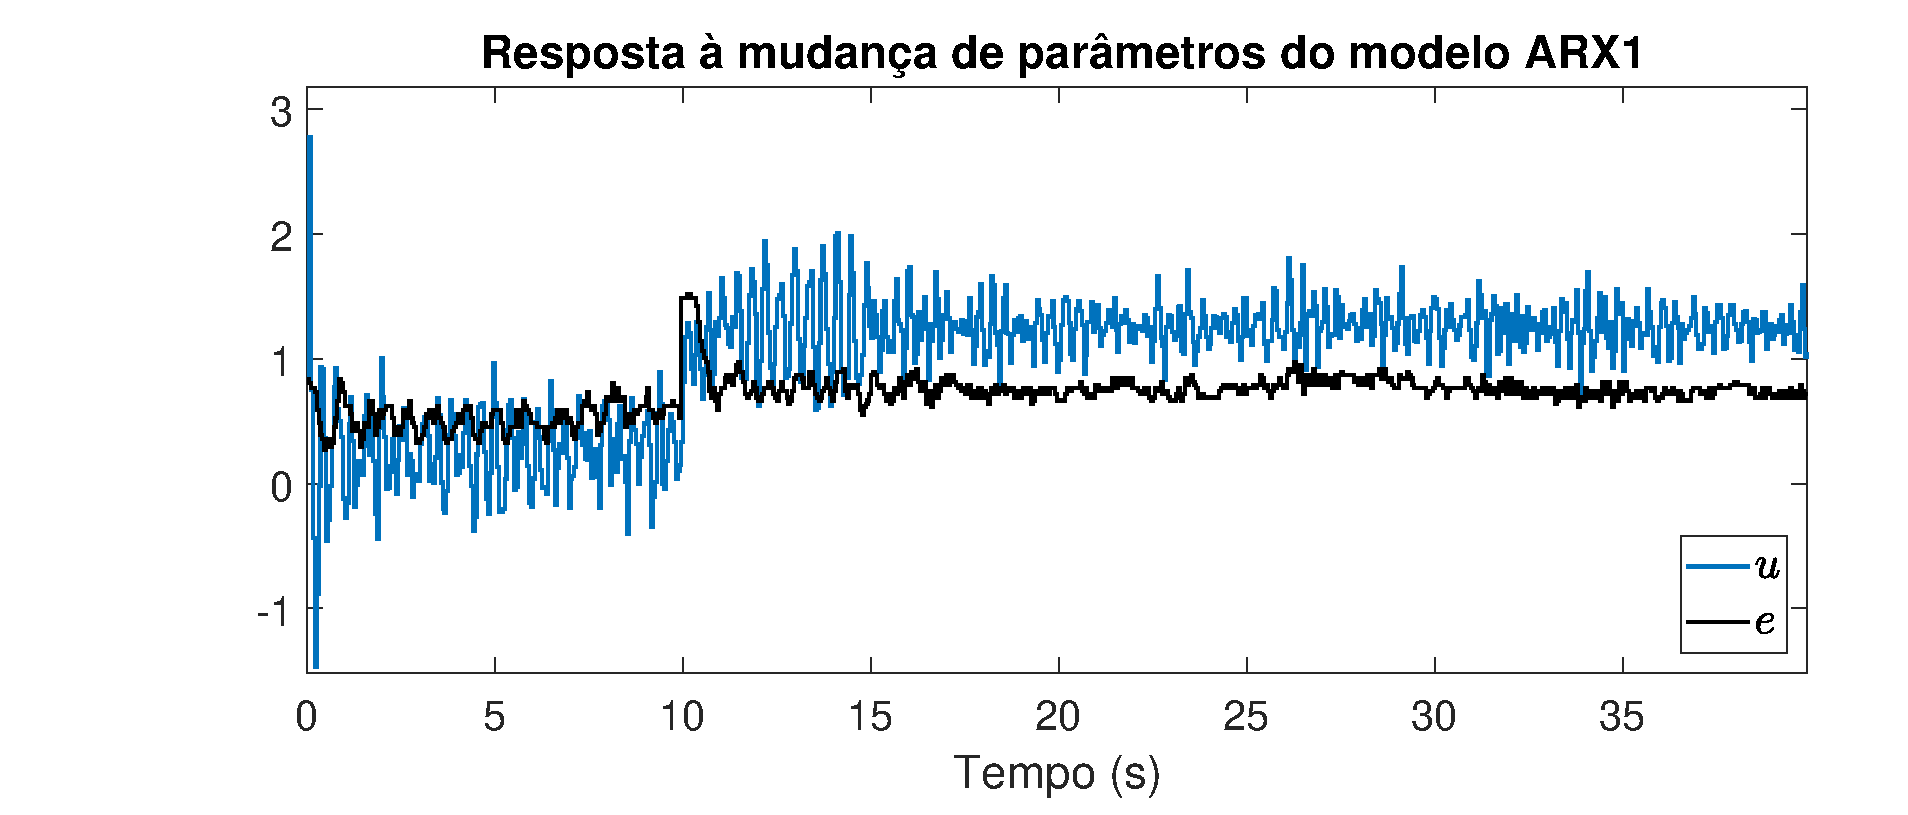
\includegraphics[width=1\linewidth]{mprarx1e}
		\caption[erro $e$ e sinal de controle $u$ do controlador $ARX1$]{erro $e$ e sinal de controle $u$ do controlador $ARX1$}
		\label{fig:mprarx1e}
	\end{subfigure}
	~ %add desired spacing between images, e. g. ~, \quad, \qquad, \hfill etc. 
	%(or a blank line to force the subfigure onto a new line)
	
	\caption{Resposta à perturbação externa do sistema com o controlador do modelo $ARX1$}\label{fig:mprarx1}
\end{figure}


\begin{figure}[H]
	\centering
	\begin{subfigure}[b]{1\textwidth}
		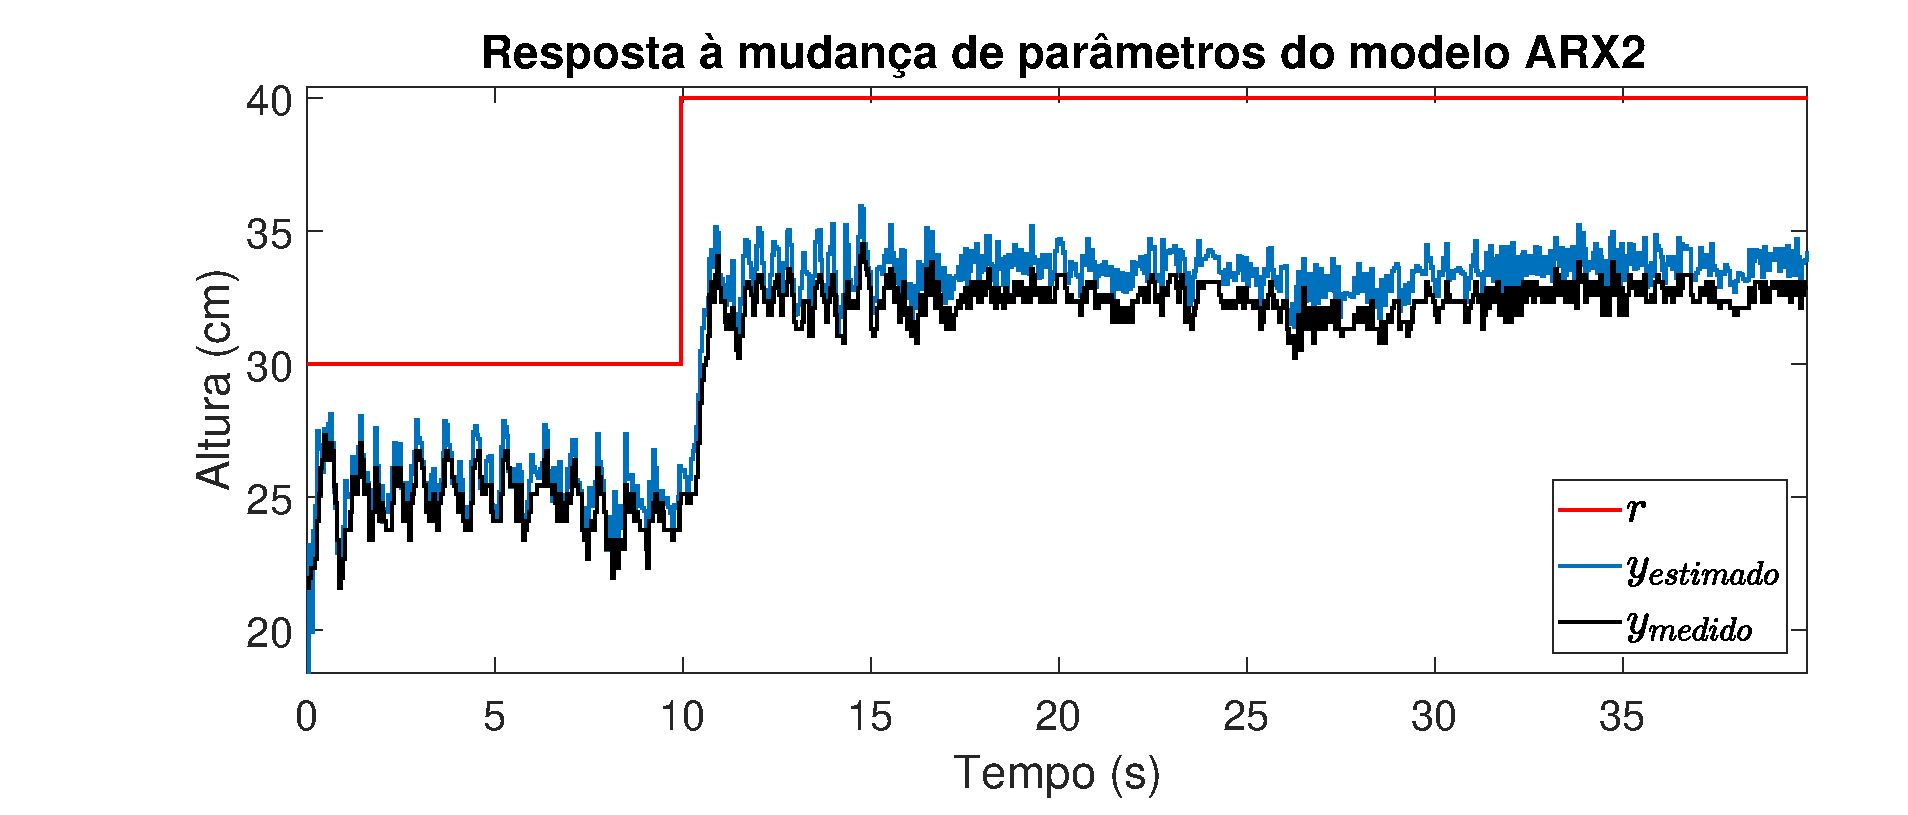
\includegraphics[width=1\linewidth]{mprarx2y}
		\caption[$y_{estimado}$ e $y_{medido}$ do modelo $ARX2$]{$y_{estimado}$ e $y_{medido}$ do modelo $ARX2$}
		\label{fig:mprarx2y}
	\end{subfigure}
	~ %add desired spacing between images, e. g. ~, \quad, \qquad, \hfill etc. 
	%(or a blank line to force the subfigure onto a new line)
	\begin{subfigure}[b]{1\textwidth}
		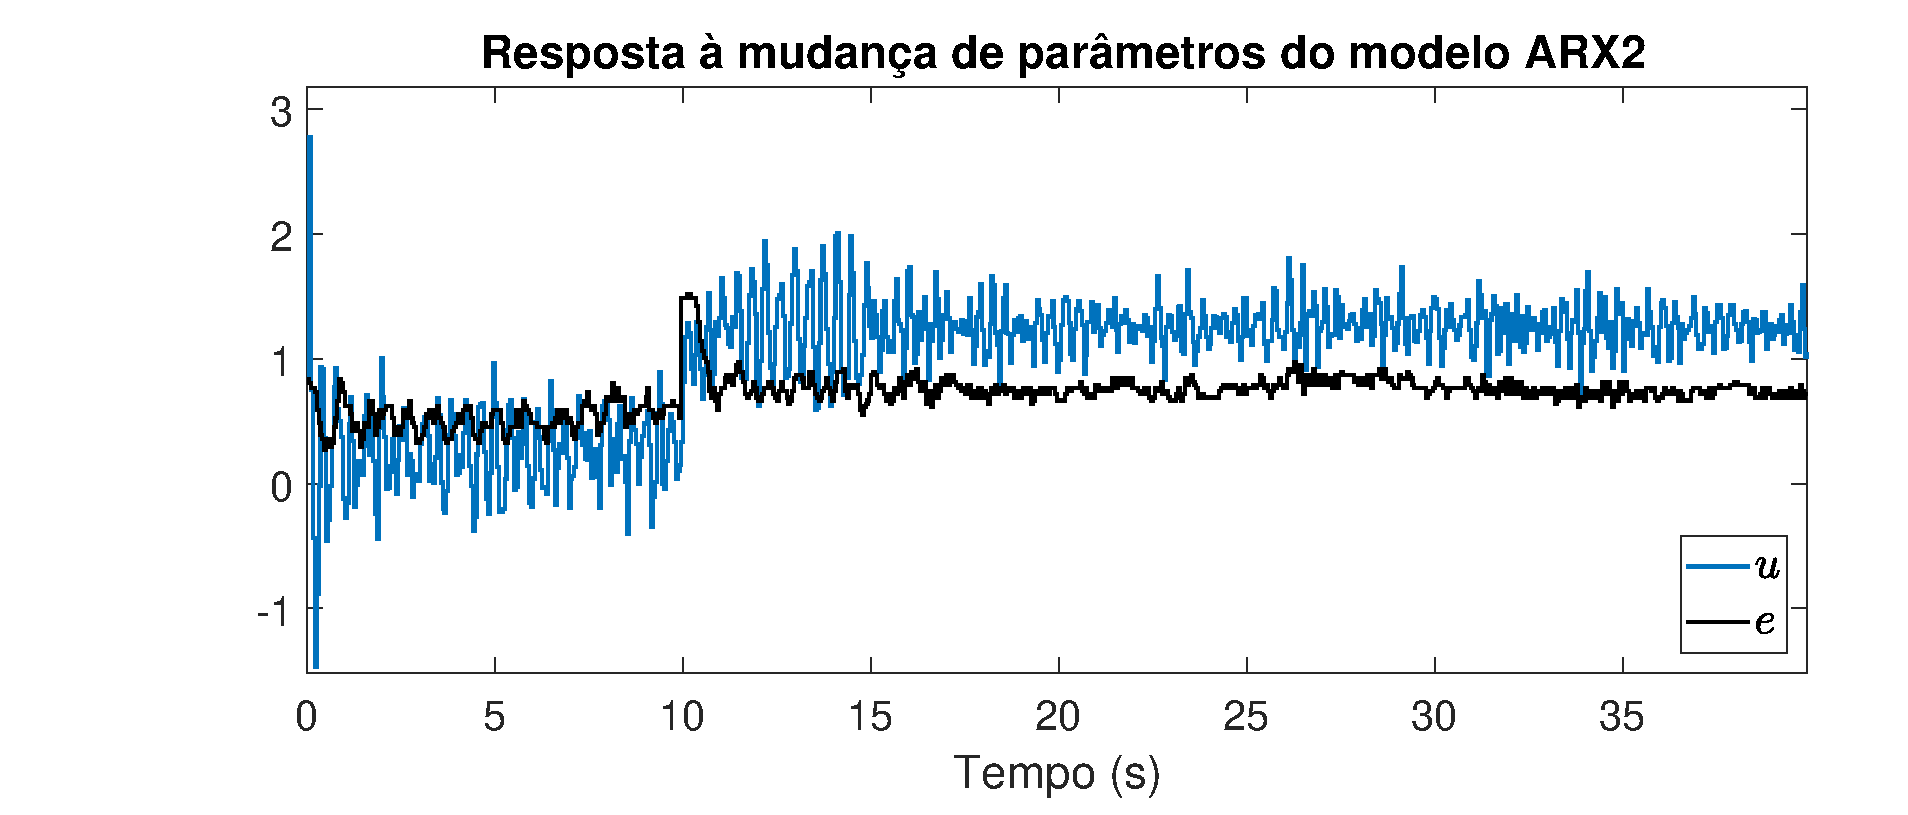
\includegraphics[width=1\linewidth]{mprarx2e}
		\caption[erro $e$ e sinal de controle $u$ do controlador $ARX2$]{erro $e$ e sinal de controle $u$ do controlador $ARX2$}
		\label{fig:mprarx2e}
	\end{subfigure}
	~ %add desired spacing between images, e. g. ~, \quad, \qquad, \hfill etc. 
	%(or a blank line to force the subfigure onto a new line)
	
	\caption{Resposta à perturbação externa do sistema com o controlador do modelo $ARX2$}\label{fig:mprarx2}
\end{figure}


\subsection{Resultados do Teste de Robustez à perturbação externa}\label{rpe}
\begin{figure}[H]
	\centering
	\begin{subfigure}[b]{1\textwidth}
		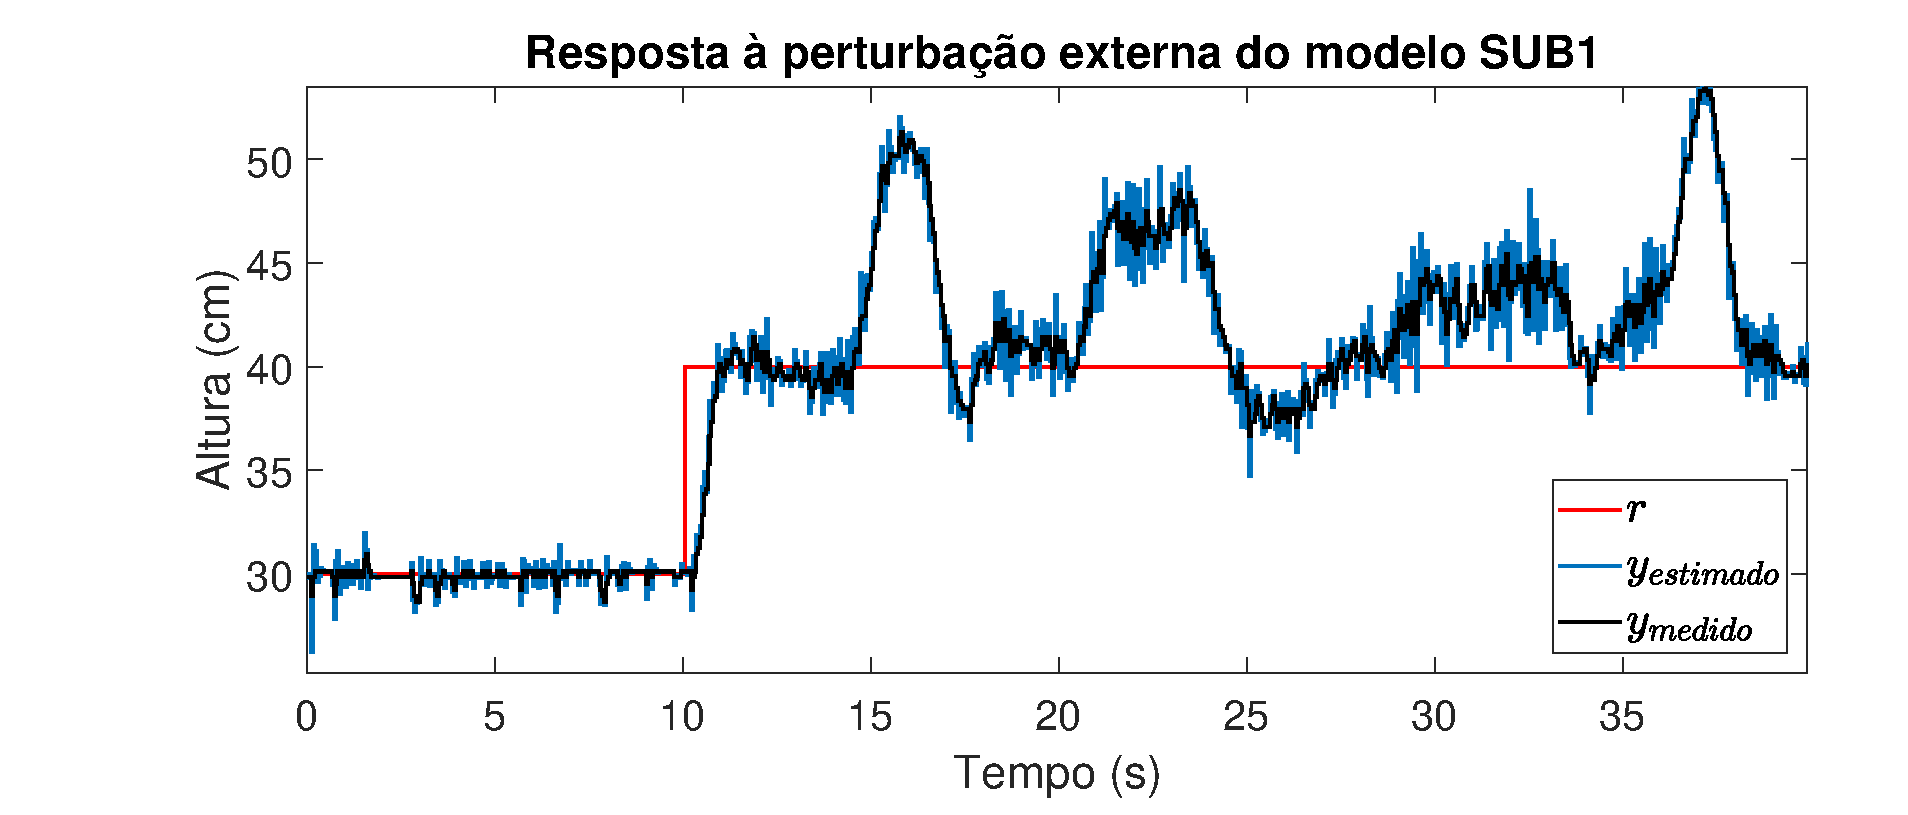
\includegraphics[width=1\linewidth]{pextrsub1y}
		\caption[$y_{estimado}$ e $y_{medido}$ do modelo $SUB1$]{$y_{estimado}$ e $y_{medido}$ do modelo $SUB1$}
		\label{fig:pextrsub1y}
	\end{subfigure}
	~ %add desired spacing between images, e. g. ~, \quad, \qquad, \hfill etc. 
	%(or a blank line to force the subfigure onto a new line)
	\begin{subfigure}[b]{1\textwidth}
		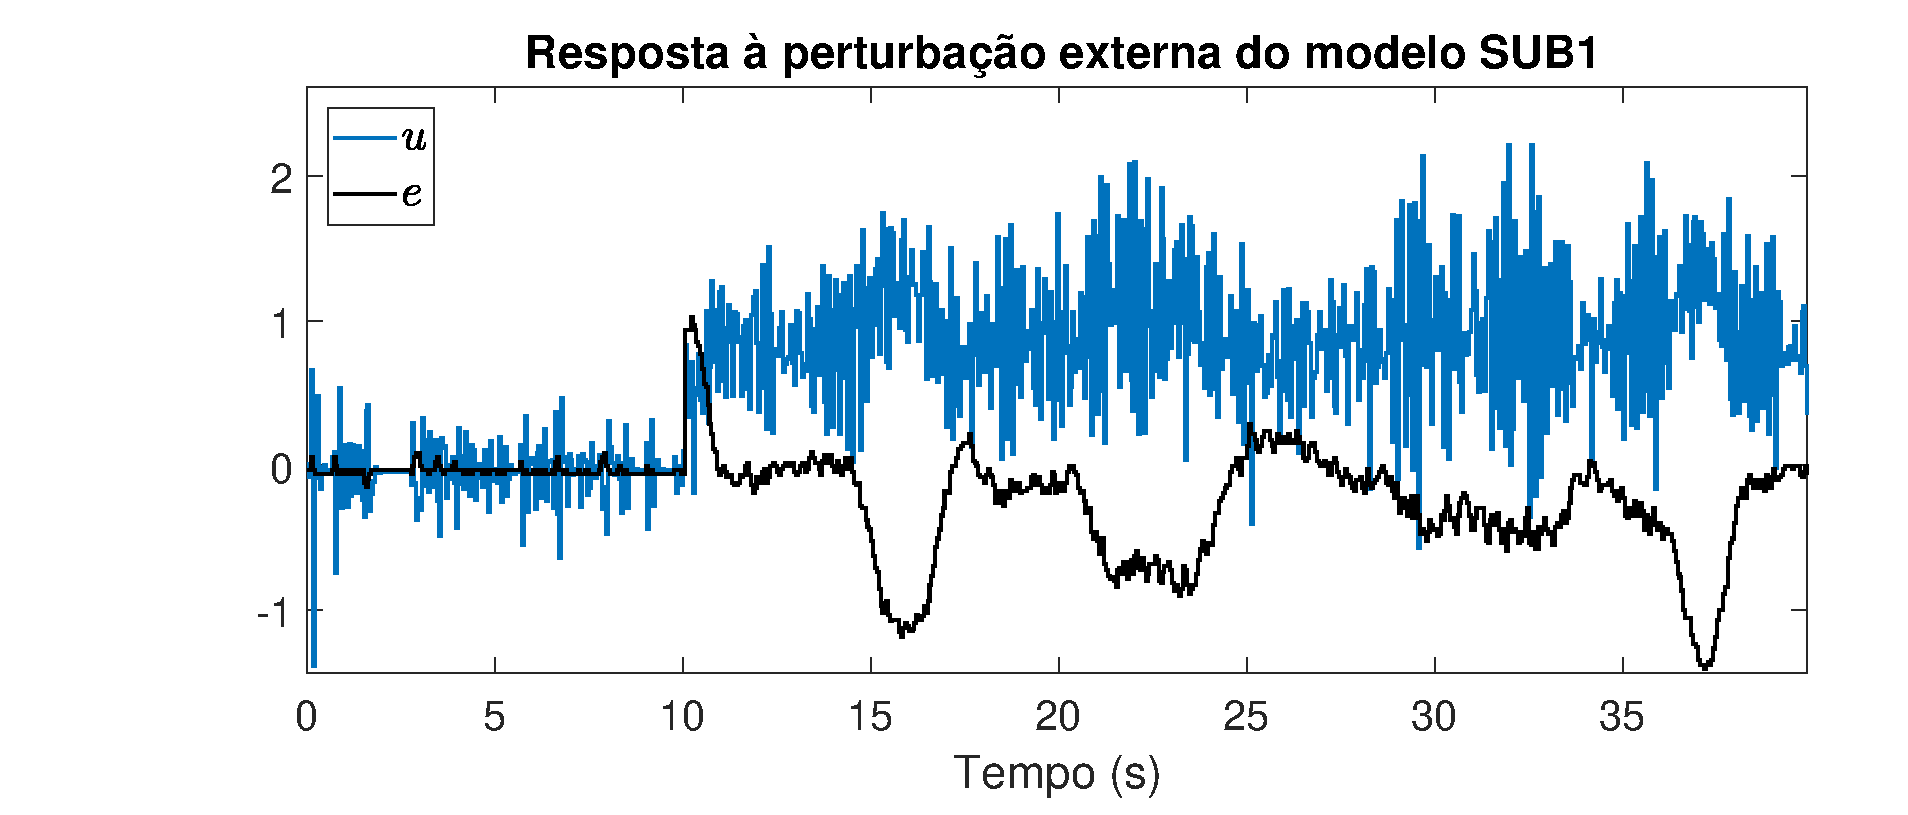
\includegraphics[width=1\linewidth]{pextrsub1e}
		\caption[erro $e$ e sinal de controle $u$ do controlador $SUB1$]{erro $e$ e sinal de controle $u$ do controlador $SUB1$}
		\label{fig:pextrsub1e}
	\end{subfigure}
	~ %add desired spacing between images, e. g. ~, \quad, \qquad, \hfill etc. 
	%(or a blank line to force the subfigure onto a new line)
	
	\caption{Resposta à perturbação externa do sistema com o controlador do modelo $SUB1$}\label{fig:pextrsub1}
\end{figure}

\begin{figure}[H]
	\centering
	\begin{subfigure}[b]{1\textwidth}
		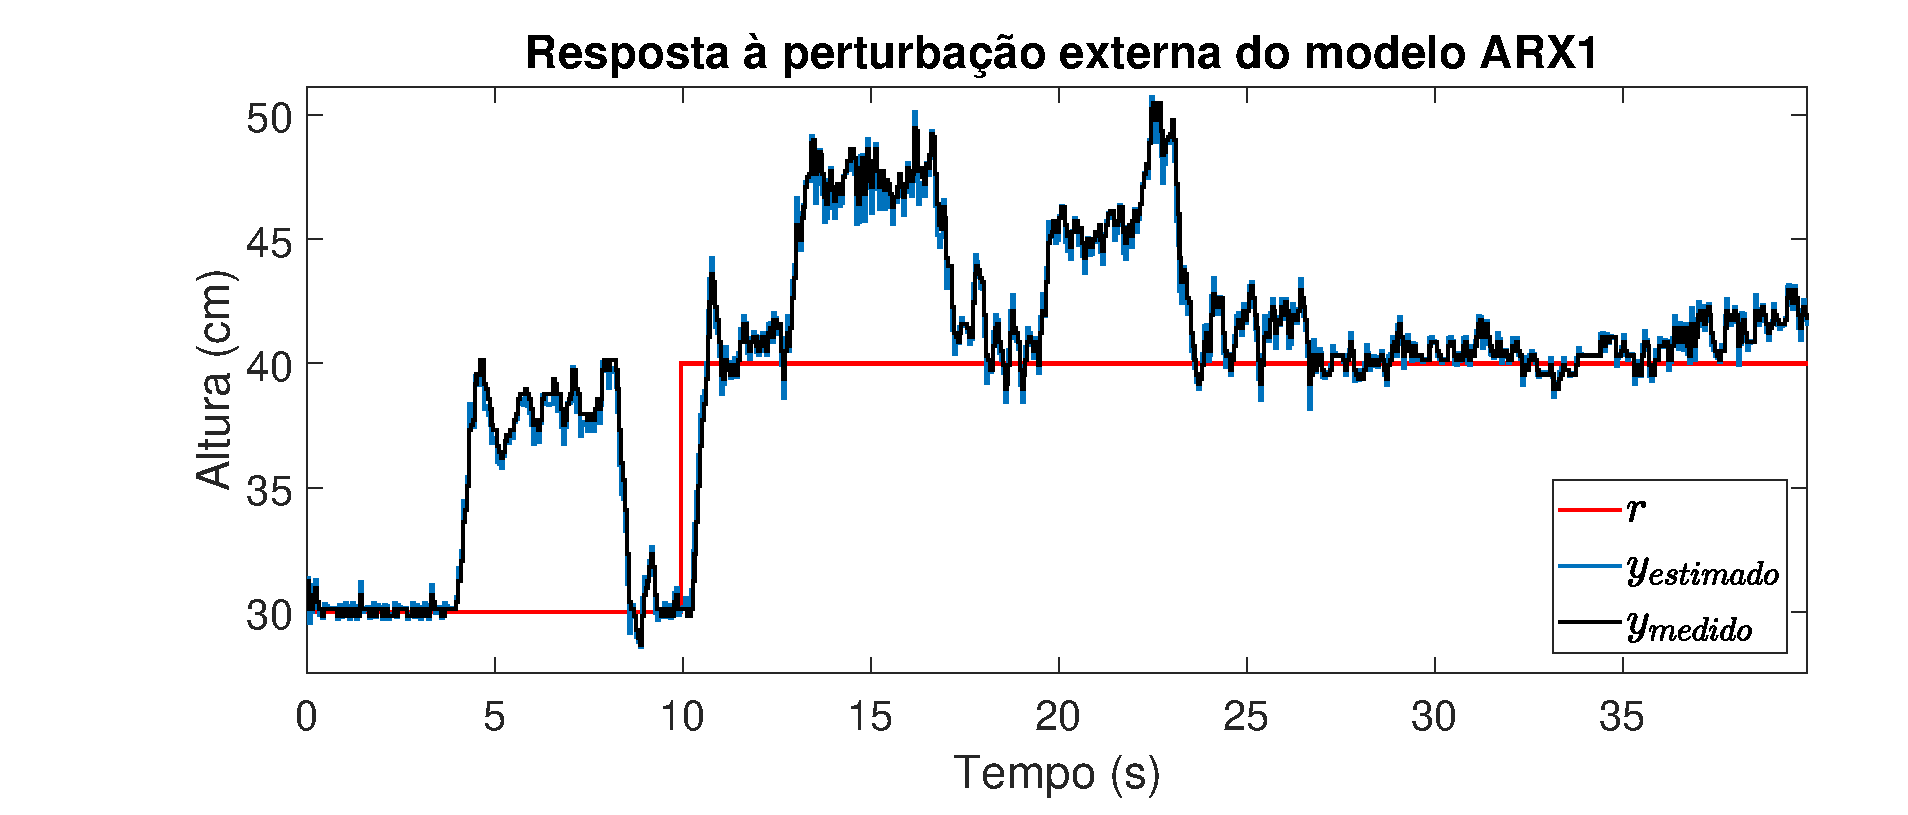
\includegraphics[width=1\linewidth]{pextrarx1y}
		\caption[$y_{estimado}$ e $y_{medido}$ do modelo $ARX1$]{$y_{estimado}$ e $y_{medido}$ do modelo $ARX1$}
		\label{fig:pextrarx1y}
	\end{subfigure}
	~ %add desired spacing between images, e. g. ~, \quad, \qquad, \hfill etc. 
	%(or a blank line to force the subfigure onto a new line)
	\begin{subfigure}[b]{1\textwidth}
		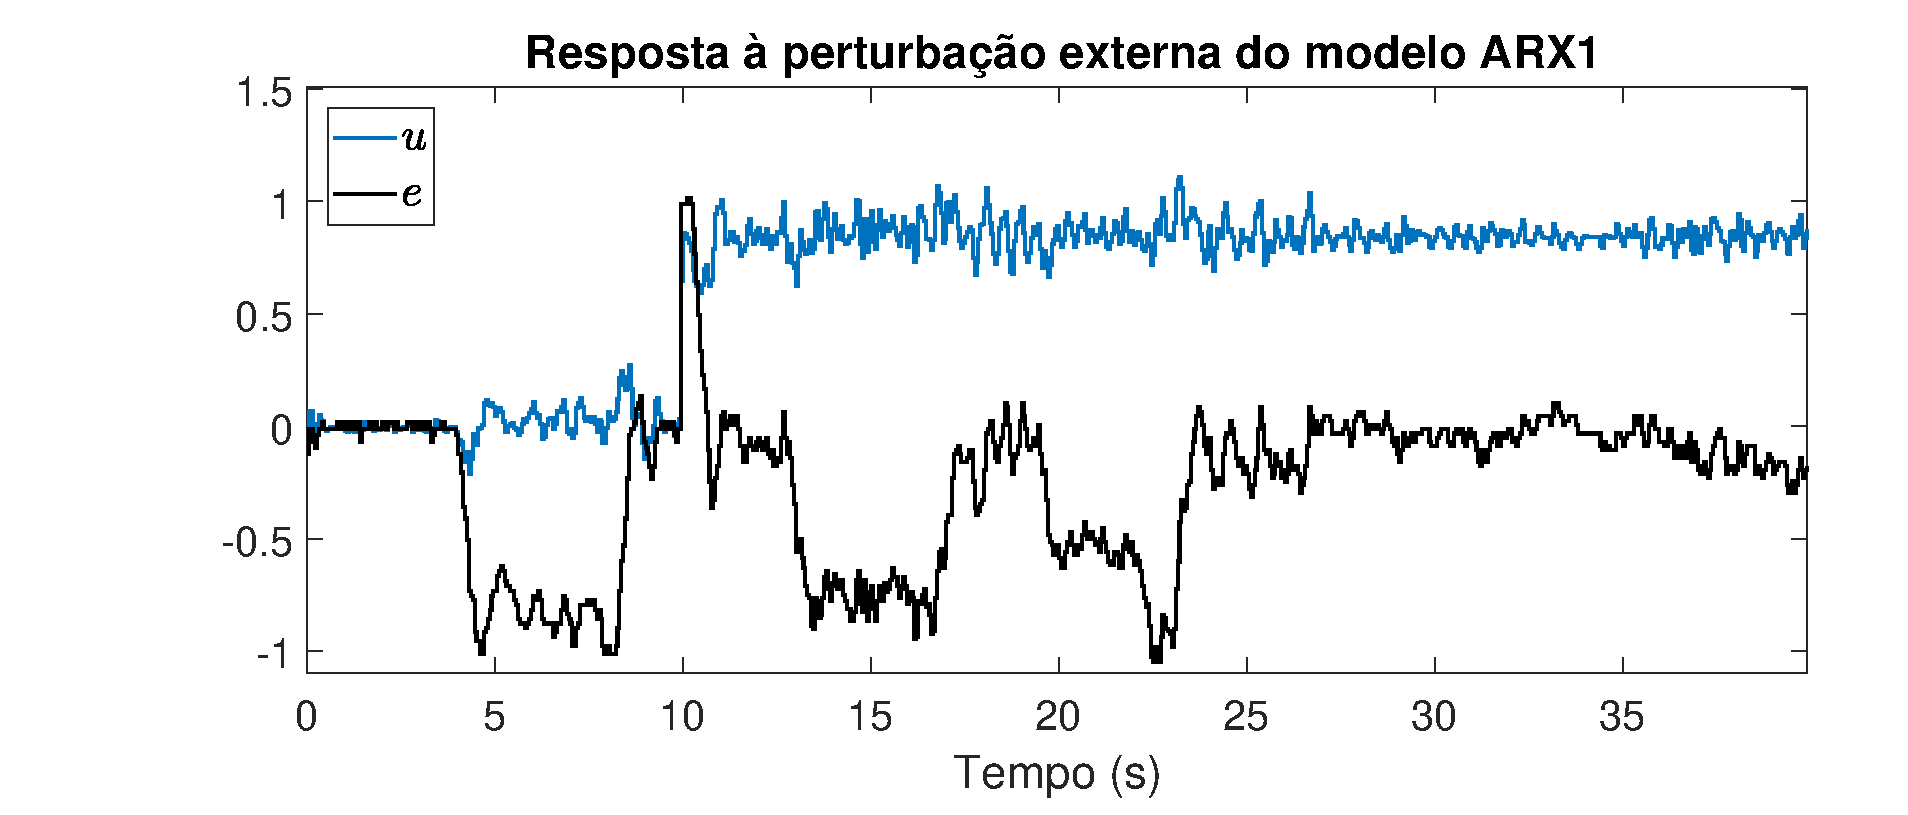
\includegraphics[width=1\linewidth]{pextrarx1e}
		\caption[erro $e$ e sinal de controle $u$ do controlador $SUB1$]{erro $e$ e sinal de controle $u$ do controlador $SUB1$}
		\label{fig:pextrarx1e}
	\end{subfigure}
	~ %add desired spacing between images, e. g. ~, \quad, \qquad, \hfill etc. 
	%(or a blank line to force the subfigure onto a new line)
	
	\caption{Resposta à perturbação externa do sistema com o controlador do modelo $ARX1$}\label{fig:pextrarx1}
\end{figure}

\begin{figure}[H]
	\centering
	\begin{subfigure}[b]{1\textwidth}
		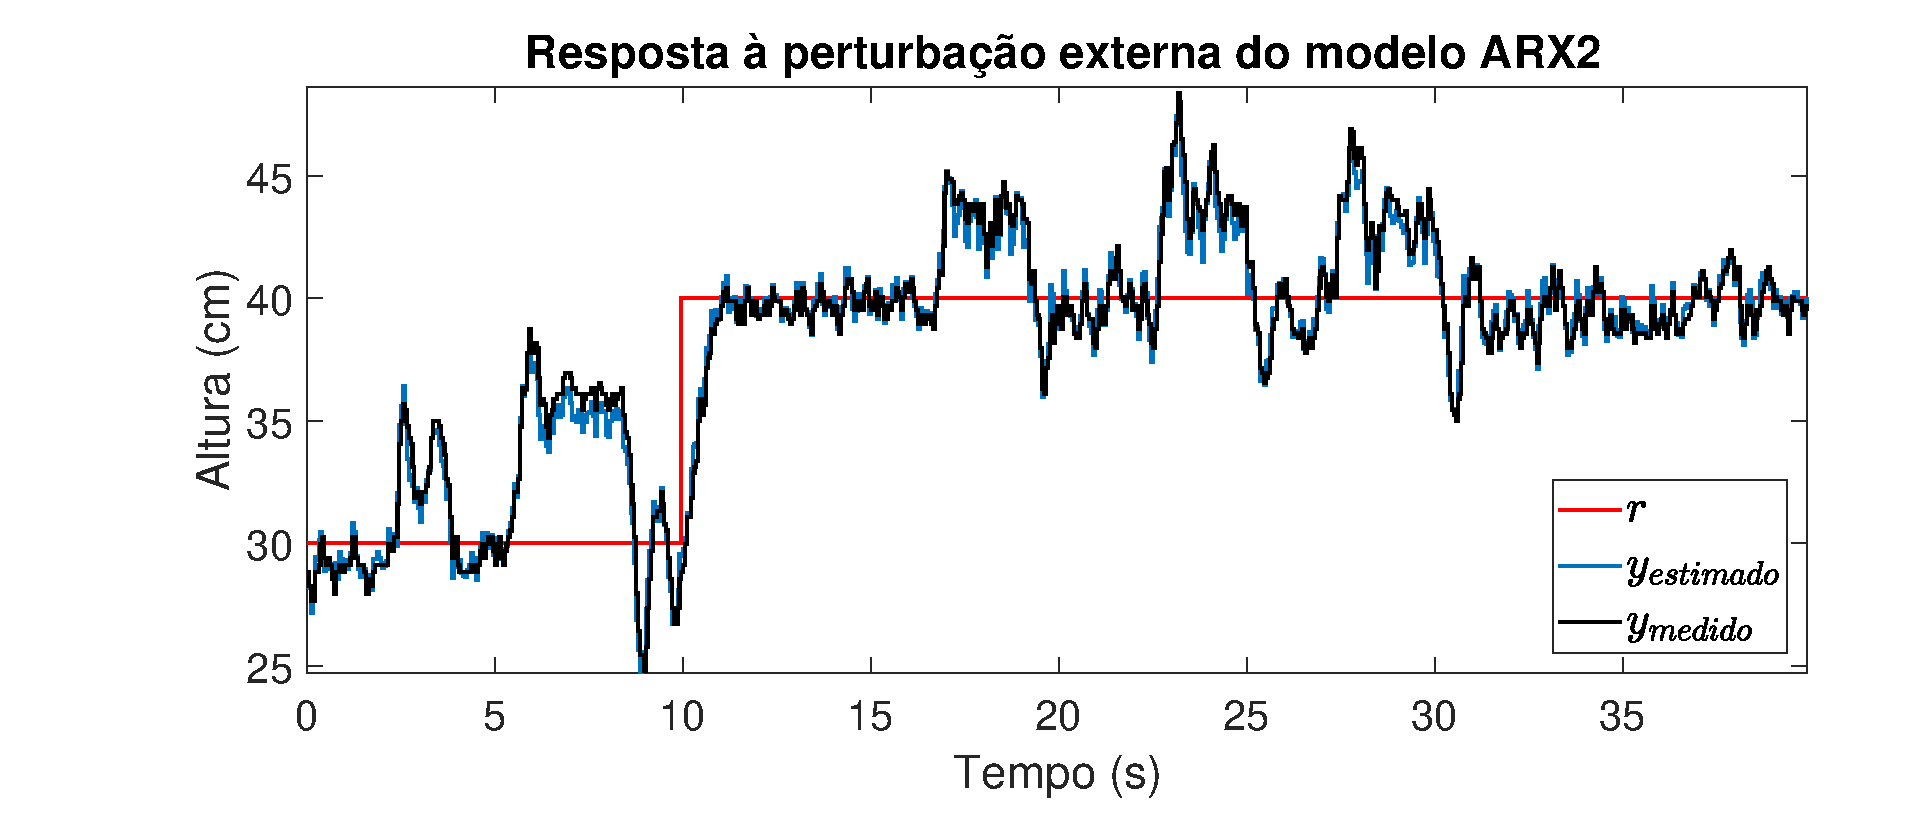
\includegraphics[width=1\linewidth]{pextrarx2y}
		\caption[$y_{estimado}$ e $y_{medido}$ do modelo $ARX2$]{$y_{estimado}$ e $y_{medido}$ do modelo $ARX2$}
		\label{fig:pextrarx2y}
	\end{subfigure}
	~ %add desired spacing between images, e. g. ~, \quad, \qquad, \hfill etc. 
	%(or a blank line to force the subfigure onto a new line)
	\begin{subfigure}[b]{1\textwidth}
		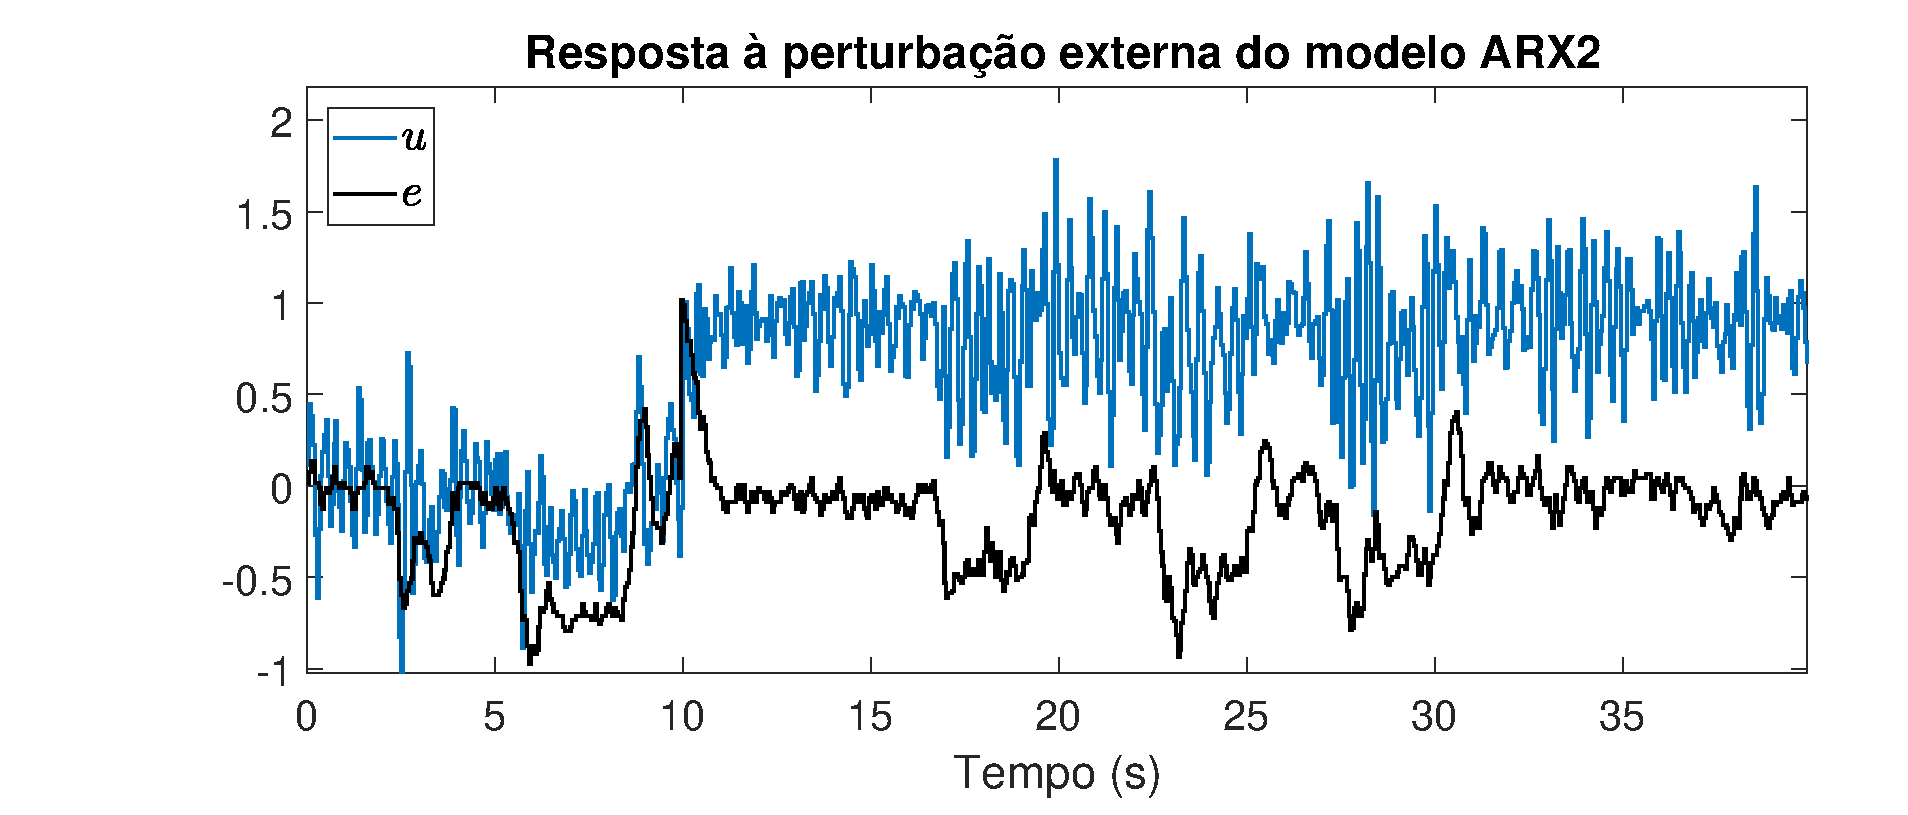
\includegraphics[width=1\linewidth]{pextrarx2e}
		\caption[erro $e$ e sinal de controle $u$ do controlador $SUB1$]{erro $e$ e sinal de controle $u$ do controlador $SUB1$}
		\label{fig:pextrarx2e}
	\end{subfigure}
	~ %add desired spacing between images, e. g. ~, \quad, \qquad, \hfill etc. 
	%(or a blank line to force the subfigure onto a new line)
	
	\caption{Resposta à perturbação externa do sistema com o controlador do modelo $ARX2$}\label{fig:pextrarx2}
\end{figure}



\section{Discussão}

Ao analisar as respostas obtidas dos experimentos devemos levar em conta o quão ruidoso é o sensor. Apesar de aplicar um filtro na saída ele ainda produz valores que apresentam um alto valor de ruído que em conjunto com o giro da bola devido a força do vento fazem com que a leitura do sensor tenha erros que influenciam nos resultados.


Nas figuras \ref{fig:steprsub1y}, \ref{fig:steprarx1y} e \ref{fig:steprarx2y} vemos em preto a saída controlada do sistema, as linhas tracejadas em preto determinam as linhas de $\pm5\%$ da referência. Com isso medimos o tempo de assentamento para eles, 8 segundos, 6 segundos, e 6 segundos, respectivamente. Nos três casos muito além do projetado na seção \ref{s:ctrl}. Isso acontece porque passamos de um modelo idealizado do sistema para o sistema real. Apesar de termos obtido um modelo adequado para representar o sistema na simulação, o controlador gerado para ele não atende as especificações quando aplicado no sistema real. É interessante notar aqui que o estimador do modelo $SUB1$ apresenta um erro maior que o estimador dos modelos $ARX1$ e $ARX2$, isso acontece porque o método dos mínimos quadrados é um método que minimiza o resíduo, e vemos isso ser passado adiante para o estimador.


Nas figuras \ref{fig:steprsub1e}, \ref{fig:steprarx1e} e \ref{fig:steprarx2e}, vemos que o sinal de controle está trabalhando para manter o erro o menor possível, apesar de não manter erro zero.


Com a seção \ref{rstair} vemos que os controladores projetados são capazes de seguir a referência dada e trabalham para reduzir o erro. Mas nas seções \ref{rmp} e \ref{rpe} fica claro que nenhum dos controladores projetados tem capacidade para reagir à mudança de parâmetros e rejeitar perturbações externas. 


Na seção \ref{s4:val} mostramos que os 3 modelos, $SUB1$, $ARX1$ e $ARX2$, identificados à partir do sistema real são adequados para representar o sistema. O modelo $ARXsim$ identificado a partir do simulador, que continha dados experimentais do sistema sobre a velocidade do vento para diferentes PWM aplicados no motor, não apresentava as características do sistema, o que fica aparente comparando as figuras \ref{fig:sinalprbsid} e \ref{fig:sinalprbsidsimul} que mostram as diferenças entre a resposta ao sinal PRBS entre os dois. O modelo $ARXsim$ também apresenta uma resposta ao degrau, figura \ref{fig:respostadegrauarxsim}, discrepante da observada no sistema real e da observada nos outros modelos obtidos.


Essa diferença nos mostra a necessidade da identificação de um sistema usando métodos caixa-preta. Apesar de termos conseguido modelar o sistema de forma matematicamente sólida, o desempenho do modelo obtido é divergente do sistema real. Enquanto que os modelos obtidos utilizando métodos de identificação caixa-preta conseguiram gerar modelos do sistema satisfatórios. 


Na seção \ref{s:ctrl} projetamos um controlador por realimentação de estados para cada um dos modelos obtidos capaz de atender as especificações de tempo de assentamento e máximo sobrevalor definidas. Mas, devido a necessidade de criar um observador de estados na seção \ref{s5:est}, vimos que a forma como o sistema modelado atende aos requisitos mudou, mesmo se mantendo dentro dos requisitos definidos. No entanto, ao aplicar esse controlador no sistema, vemos que a resposta não está atendendo aos requisitos estabelecidos. Projetamos ainda um controlador para o modelo obtido do simulador, identificado por caixa-cinza, e ao aplicarmos no sistema real a resposta foi instável, reforçando a necessidade de obter modelos por identificação caixa-preta.


Vemos que os estimadores dos dois modelos ARX ao serem aplicados no sistema tem um bom desempenho, figuras \ref{fig:erroarx1} e \ref{fig:erroarx2}, permanecendo abaixo de 1 cm de diferença com algumas exceções, que atribuímos ao ruído do sensor. O estimador do modelo $SUB1$ não apresenta bom desempenho mostrando erros superiores a 1cm com frequência.








